\documentclass[aps,floatfix,10pt,amssymb,amsfont,amsmath,superscriptaddress,float,nofootinbib,longbibliography,nobalancelastpage,twocolumn]{revtex4-2}
\usepackage{graphicx} % Required for inserting images
\usepackage{hyperref}
\usepackage{braket}
\usepackage{amsfonts}
\usepackage{amssymb}
\usepackage{amsmath}
\usepackage{bbm}
\usepackage{bm}
\usepackage[english]{babel}
\usepackage{amsthm}
\newtheorem{theorem}{Theorem}
\newtheorem{lemma}{Lemma}
\newtheorem{duplicate}{Theorem}
\newtheorem{corollary}{Corollary}
\usepackage{subfig}
\usepackage{tikz}
\usetikzlibrary{arrows,positioning}
 \usetikzlibrary{quotes}
\usepackage{yquant}
\pgfdeclareshape{yquant-multictrlshape}{
   \inheritsavedanchors[from=yquant-circle]%
   \foreach \anc in {center, north, north east, east, south east, south, south west, west, north west} {%
      \inheritanchor[from=yquant-circle]{\anc}%
   }%
   \inheritanchorborder[from=yquant-circle]%
   \backgroundpath{%
      \pgfpathmoveto{\pgfqpoint{-0.707107\dimexpr\xradius\relax}{-0.707107\dimexpr\yradius\relax}}%
      \pgfpathlineto{\pgfqpoint{0.707107\dimexpr\xradius\relax}{0.707107\dimexpr\yradius\relax}}%
      \pgfpathellipse{\pgfpointorigin}%
                     {\pgfqpoint{\xradius}{0pt}}%
                     {\pgfqpoint{0pt}{\yradius}}%
   }%
   \inheritclippath[from=yquant-circle]%
}

\yquantset{multictrl/.style={every negative control/.style={draw, /yquant/default fill,shape=yquant-multictrlshape,radius=1.05mm}}}
\pgfdeclareshape{yquant-bctrlshape}{
   \inheritsavedanchors[from=yquant-circle]%
   \foreach \anc in {center, north, north east, east, south east, south, south west, west, north west} {%
      \inheritanchor[from=yquant-circle]{\anc}%
   }%
   \inheritanchorborder[from=yquant-circle]%
   \backgroundpath{%
      % Draw the circle
      \pgfpathellipse{\pgfpointorigin}%
                     {\pgfqpoint{\xradius}{0pt}}%
                     {\pgfqpoint{0pt}{\yradius}}%
   }%
   % Add the "b" in the center
   \foregroundpath{%
      \pgftext[center]{\(\scriptstyle b\)}%
   }%
   \inheritclippath[from=yquant-circle]%
}

\yquantset{
  bctrl/.style={
    every control/.style={
      draw,
      /yquant/default fill,
      shape=yquant-bctrlshape,
      radius=1.05mm
    }
  }
}
\date{February 2025}
\begin{document}
\yquantdefinebox{dots}[inner sep=0pt]{$\dots$}

\title{New and Improved Quantum Metropolis Sampling}
\author{Oliver O'Brien}
\affiliation{Department of Applied Mathematics and Theoretical Physics, University of Cambridge,\\ Wilberforce Road, Cambridge, CB3 0WA, United Kingdom}
\author{Rakesh Achutha}
\affiliation{Department of Applied Mathematics and Theoretical Physics, University of Cambridge,\\ Wilberforce Road, Cambridge, CB3 0WA, United Kingdom}
\author{Frank Verstraete}
\affiliation{Department of Applied Mathematics and Theoretical Physics, University of Cambridge,\\ Wilberforce Road, Cambridge, CB3 0WA, United Kingdom}
\affiliation{Department of Physics and Astronomy, Ghent University, Krijgslaan 281, 9000 Gent, Belgium}

\begin{abstract}
    We introduce a resource-efficient protocol for Boosted State-Independent Quantum Phase Estimation (BSI-QPE), enabling practical implementation of the Quantum Metropolis algorithm. By employing window functions to suppress fat tails, our approach maintains coherence and shift invariance required for reversible sampling. We reframe the rejection process using a two-dimensional invariant subspace. A modified formulation of approximate quantum detailed balance is proposed, ensuring convergence to Gibbs states under realistic error bounds. These advancements significantly lower the resource threshold for quantum thermal state preparation.
\end{abstract}

\maketitle

\section{Introduction}
The Quantum Metropolis algorithm, first proposed by Temme et al. \cite{Temme_2011}, remains one of the most promising quantum algorithms for sampling from Gibbs (thermal) states of quantum systems. These states are fundamental in statistical mechanics and appear across condensed matter physics, quantum chemistry, and high-energy physics, where accurate thermal state preparation is a central computational challenge. 

However, the algorithm as originally stated suffers from two major issues which have led the community to investigate alternative gibbs sampling techniques (\cite{}). Firstly, \cite{Temme_2011} heavily relies upon phase estimation and hence has to deal with the resultant fat tails \cite{}.  Numerous solutions to this problem have been explored (\cite{}). In the original paper \cite{Temme_2011} it was posited that coherently taking the median of multiple phase estimations could help boost the signal and remove these fat tails. However, the phase estimation is also required to be shift invariant which the median trick struggles to fulfill. Recently, \cite{chen2023quantumthermalstatepreparation} proved a no-go theorem suggesting that it is not possible to implement the boosted shift-invariant phase estimation required by the quantum metropolis algorithm. 

We propose a boosted shift-invariant phase estimation protocol which utilises window functions to exponentially dampen the fat tails. This drastically reduces the number of ancilla qubits required for the algorithm to work, and also conclusively proves that quantum metropolis does indeed work. 

In Section \ref{section:boostedphaseestimation} we present the construction of the Boosted Shift-Invariant Quantum Phase Estimation (BSI-QPE) protocol, including a detailed circuit-level description and error analysis based on window functions. In Section \ref{section:algorithm}, we describe our modified Quantum Metropolis algorithm incorporating our improved quantum phase estimation. This includes a novel understanding of the rewinding mechanism formulated through iterative projective measurements and invariant subspaces. Section \ref{section:why} rigorously proves that our algorithm satisfies an approximate quantum detailed balance condition and discusses the convergence guarantees to the thermal Gibbs state. Finally, in Section \ref{section:discussion}, we discuss the broader implications of our results, the assumptions made, and the outlook for implementing these techniques on near-term or fault-tolerant quantum hardware.


\section{Boosted State-Independent Quantum Phase Estimation}
\label{section:boostedphaseestimation}
Given an $m$-qubit Hamiltonian $H$ eigenvectors $\ket{\psi_j}$ such that $H\ket{\psi_j} = E_j \ket{\psi_j}$, quantum phase estimation (QPE) allows one to prepare an ancilla register that approximates $E_j$. Unfortunately, quantum computers have limited precision. As a result, unless the energy can be represented exactly in binary using $\eta$ bits (corresponding to $\eta$ ancilla qubits), there is a high probability of obtaining an inaccurate energy measurement. This inaccuracy arises from the ``fat tails" in QPE \cite{}. 

Often this issue can be mitigated by simply repeating the calculation and taking an average. However, quantum metropolis sampling requires us to ``rewind" upon rejecting a proposed update and hence we require a unitary method for ``boosting" QPE. This ``boosted" QPE stores an approximation to the energy in ancillas which is not immediately measured but rather used as the basis for further coherent calculations. Further, for ``rewinding" to work we must reuse the same ancilla registers so the QPE protocol must also be state-independent. Therefore, we must demonstrate an implementation of a boosted state-independent quantum phase estimation (BSI-QPE). While it has been shown \cite{chen2023quantumthermalstatepreparation} that QPE cannot entirely eliminate the probability mass in its tails, we demonstrate that it is possible to construct BSI-QPE protocols with exponentially suppressed tails, which effectively mitigate the issue for practical purposes. 

Existing methods for boosting QPE rely upon choosing specific input ancillary states. In these methods QPE is performed using ancillas initialised to the state $\sum_x \alpha(x) \ket{x}$ for some window function $\alpha(x)$ instead of the standard uniform superposition. After performing QPE upon eigenstate $\ket{\psi_j}$ the following state is produced:
\begin{equation}
   \frac{1}{\sqrt{2^{\eta}}} \sum_x \sum_k e^{\frac{2 \pi i}{2^{\eta}}x(k-E_j)} \alpha(x)\ket{k}\ket{\psi_j}
\end{equation}
which can be rewritten as:
\begin{equation}
    \sum_k \hat\alpha(k-E_j) \ket{k}\ket{\psi_j}
\end{equation}
where $\hat \alpha(k)$ is the discrete fourier transform of $\alpha(x)$. By choosing $\alpha$ to be a window function one can ensure that $\hat \alpha$ is narrowly peaked, thus QPE is boosted. Unfortunately, this is not sufficient for the quantum metropolis algorithm as we require the QPE to be independent of the ancillary state, as we must reuse the same ancillas throughout the rewinding process. 

Our construction uses two window functions $\alpha(x)$ and $\beta(x) = \sqrt{1-\alpha(x)^2}$ (for $x\in\{0,1,\ldots,2^{\eta}-1\}$) which are both narrowly peaked in the fourier domain. We introduce these windows via the following multi-controlled single-qubit rotation:
\begin{equation}
   CR_Y = \sum_k \ket{k}\bra{k}\otimes \begin{pmatrix}
        \alpha(k)& \beta(k)\\
        -\beta(k)& \alpha(k)
    \end{pmatrix}
\end{equation}

We also require the following time evolution gadget which is constructed as shown in Fig~\ref{fig:CRZ}:
\begin{equation}
    CR_Z =\sum_{j,k}\ket{\psi_j}\bra{\psi_j}\otimes\ket{k}\bra{k} \otimes \begin{pmatrix}
        e^{\frac{iE_jkt}{2}}&0\\
        0 & e^{-\frac{iE_jkt}{2}}
    \end{pmatrix}
\end{equation}
\begin{figure*}
\vcenter{\hbox{
\resizebox{!}{2.5cm}{
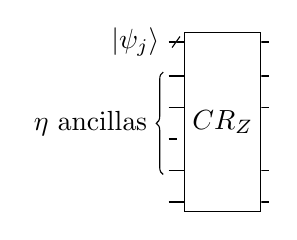
\begin{tikzpicture}
\begin{yquant*}
qubit {$\ket{\psi_j}$} s;

init {$\eta$ ancillas} (a[0,1],ellipsis, aend);
slash s;
hspace {0.1cm} -;
discard ellipsis;
% qubit {} aend;
qubit {} f;
box {$CR_Z$} (s,a,ellipsis, aend, f);

% text {$\ket{0}$} f;
\end{yquant*}
\end{tikzpicture}}}}
=
\vcenter{\hbox{
\resizebox{!}{2.5cm}{
    \begin{tikzpicture}
\begin{yquant*}
qubit {$\ket{\psi_j}$} s;

init {$\eta$ ancillas} (a[0,1],ellipsis, aend);
discard ellipsis;
% qubit {} aend;
qubit {} f;
slash s;
hspace {0.1cm} -;

box {$U^{\dagger 2^0}$} (s) | a[0], f;
box {$U^{\dagger 2^1}$} (s) | a[1], f;
hspace {0mm} -;
dots ellipsis;

box {$U^{\dagger 2^{\eta-1}}$} (s) | aend[0], f;
box {$U^{2^0}$} (s) | a[0]~ f;
box {$U^{ 2^1}$} (s) | a[1]~ f;
hspace {0mm} -;
dots ellipsis;

box {$U^{ 2^{\eta-1}}$} (s) | aend[0]~ f;
\end{yquant*}
\end{tikzpicture}}}}
\caption{Quantum circuit for implementing an $Z$ rotation on an ancilla qubit that is dependent upon the energy of the system. The unitary $U=e^{\frac{iHt}{2}}$ is implemented through some quantum time evolution algorithm (e.g. trotterisation \cite{lloyd1996universal}, qubitization \cite{Low2019hamiltonian}) up to an operator norm error of $\epsilon^T_t$. Throughout this work we assume  $\epsilon^T_t$ is negligible, and use perfect quantum time evolution in our error analysis.}
    \label{fig:CRZ}
\end{figure*}
Both of these act as controlled $R_Z$ and $R_Y$ rotations on a single qubit. 
\begin{figure*}
\vcenter{\hbox{
\resizebox{!}{2.5cm}{
\begin{tikzpicture}
    \begin{yquant*}
qubit {$\ket{\psi_j}$} s;

init {$\eta$ ancillas} (a[0,1],ellipsis, aend);
slash s;
% hspace {0.1cm} -;
discard ellipsis;
% qubit {} aend;
qubit {} f;
dots ellipsis;

box {BSI-\\QPE} (s,a,ellipsis, aend, f);

% text {$\ket{0}$} f;
\end{yquant*}
\end{tikzpicture} }}}
=
\vcenter{\hbox{
\resizebox{!}{2.5cm}{
\begin{tikzpicture}
    \begin{yquant*}
qubit {$\ket{\psi_j}$} s;

init {$\eta$ ancillas} (a[0,1],ellipsis, aend);
slash s;
discard ellipsis;
% qubit {} aend;
qubit {} f;
dots ellipsis;
box {QFT} (a,ellipsis, aend);

[this subcircuit box style={dashed, "$R_Z[E_jt(k-k')]$"}]
subcircuit {
qubit {} s;
qubit {} a[2];
qubit {} ellipsis;
qubit {} aend;
discard ellipsis;
qubit {} f;

% dots ellipsis;
box {$CR_Z$} (s,a,ellipsis, aend, f);

x aend[0];
dots ellipsis;
box {$CR_Z^{\dagger}$} (s,a,ellipsis, aend, f);
x aend[0];
dots ellipsis;
} (s,a,ellipsis, aend, f);

box {$CR_Y$} (a,ellipsis, aend, f);

[this subcircuit box style={dashed, "$R_Z[E_jt(k+k'-2^{\eta})]$"}]
subcircuit {
qubit {} s;
qubit {} a[2];
qubit {} ellipsis;
qubit {} aend;
discard ellipsis;
qubit {} f;

box {$CR_Z$} (s,a,ellipsis, aend, f);
x aend[0];
dots ellipsis;
box {$CR_Z$} (s,a,ellipsis, aend, f);
x aend[0];
dots ellipsis;
box {$U^{\dagger 2^{\eta}}$} (s) ~ f;
box {$U^{2^{\eta}}$} (s) | f;
} (s,a,ellipsis, aend, f);

box {iQFT} (a,ellipsis, aend);

% text {$\ket{0}$} f;
\end{yquant*}
\end{tikzpicture} }}}

\caption{Quantum circuit implementing boosted state-independent quantum phase estimation (BSI-QPE). We highlight how the combinations of $CR_Z$ and $X$ gates operators correspond to the single qubit $R_Z$ given in Eq.~\ref{eq:euler} with $k$ being the value stored in the $\eta$ ancillas and $k' = k + 2^{\eta-1} \mod 2^{\eta}$}
\label{fig:circuit}
\end{figure*}
\begin{figure*}
\begin{tikzpicture}
    \begin{yquant*}
qubit {$\ket{\psi_j}$} s;

init {$\eta$ ancillas} (a[0,1],ellipsis, aend);
slash s;
discard ellipsis;
% qubit {} aend;
dots ellipsis;
box {QFT} (a,ellipsis, aend);

box {$U^{ 2^1}$} (s) | a[0];
box {$U^{ 2^2}$} (s) | a[1];
hspace {0mm} -;
dots ellipsis;

box {$U^{ 2^{\eta}}$} (s) | aend[0];
box {$U^{\dagger 2^{\eta}}$} (s);
box {iQFT} (a,ellipsis, aend);

% text {$\ket{0}$} f;
\end{yquant*}
\end{tikzpicture} 

\caption{Quantum circuit implementing unboosted state-independent QPE with $U=e^{\frac{iHt}{2}}$, equivalent to choosing $\alpha(x)=1$ for BSI-QPE. This slightly differs from the standard formulation of QPE \cite{Nielsen_Chuang_2010} by beginning with $QFT$ rather than $H^{\otimes \eta}$ and the addition of $U^{\dagger 2^{\eta}}$ at the end. }
\label{fig:standard_qpe}
\end{figure*}

\begin{widetext}
We can implement BSI-QPE through the circuit illustrated in Fig~\ref{fig:circuit}. This circuit combines the  $CR_Z$ and $CR_Y$ rotations using the following $R_ZR_YR_Z$ decomposition \cite{Nielsen_Chuang_2010}: 
\begin{equation}
\label{eq:euler}
    R_Z[E_jt(k+k'-2^{\eta})]R_Y[2\arccos(\alpha(k))]R_Z[E_jt(k-k')] = \begin{pmatrix}
        \alpha(k)e^{iE_jtk}e^{-iE_jt2^{\eta-1}} && \beta(k)e^{iE_jt k'}e^{-iE_jt2^{\eta-1}}\\
        -\beta (k)e^{-iE_jt k'}e^{iE_jt2^{\eta-1}} && \alpha(k)e^{-iE_jtk}e^{iE_jt2^{\eta-1}}
    \end{pmatrix}
\end{equation}
In Fig.~\ref{fig:circuit}, the $X$-gates acting on the last qubit in the ancilla register shift the value stored from $k$ to $k'= k+2^{\eta-1} \mod 2^{\eta}$, and hence we get the following operation:
\begin{multline}
        \text{BSI-QPE} = \frac{1}{2^{\eta}}\sum_j\sum_{p,q,k} \begin{pmatrix}
        \alpha(k)e^{iE_jtk}e^{-iE_jt2^{\eta-1}} && \beta(k)e^{iE_jt[(k+2^{\eta-1})\text{mod} 2^{\eta}]}e^{-iE_jt2^{\eta-1}}\\
        -\beta (k)e^{-iE_jt[(k+2^{\eta-1})\text{mod} 2^{\eta}]}e^{iE_jt2^{\eta-1}} && \alpha(k)e^{-iE_jtk}e^{iE_jt2^{\eta-1}}
    \end{pmatrix}e^{\frac{2\pi i}{2^{\eta}}k(q-p)} \\\otimes\ket{p}\bra{q}\otimes\ket{\psi_j}\bra{\psi_j}
\end{multline}
This can be simplified to:
\begin{equation}
    \text{BSI-QPE} = \frac{1}{\sqrt{2^{\eta}}}\sum_j\sum_{p,q} \begin{pmatrix}
        (-1)^{q-p}\hat\alpha(q-p+\frac{2^{\eta}}{2\pi}E_jt) && \hat\beta(q-p+\frac{2^{\eta}}{2\pi}E_jt)\\
        -\hat\beta (q-p-\frac{2^{\eta}}{2\pi}E_jt) && (-1)^{q-p}\hat\alpha(q-p-\frac{2^{\eta}}{2\pi}E_jt)
    \end{pmatrix}\otimes\ket{p}\bra{q}\otimes\ket{\psi_j}\bra{\psi_j}
\end{equation}
% \begin{multline}
%   \sum_j \sum^{2^{\eta}}_{p,q} \hat \alpha(p - q - \frac{2^{\eta} t}{2\pi}E_j)\ket{0}\bra{0} \otimes\ket{p}\bra{q} \otimes \ket{\psi_j} \bra{\psi_j}\\
%   + \ket{0}\bra{0} \otimes\bm{\varepsilon}^T_{kt}
% \end{multline}
where $\hat \alpha$ is the discrete fourier transform of $\alpha$ as given by:
\begin{equation}
   \hat\alpha(x) =\frac{1}{\sqrt{2^{\eta}}}\sum_{k=-2^{\eta-1}}^{2^{\eta-1}-1} \alpha(k+2^{\eta-1})e^{\frac{2\pi i}{2^{\eta}}xk}
\end{equation}
and $\hat \beta$ is the discrete fourier transform of $\beta$ given by:
\begin{equation}
    \hat\beta(x) =\frac{1}{\sqrt{2^{\eta}}}\sum_{k=-2^{\eta-1}}^{2^{\eta-1}-1} \beta(k)e^{\frac{2\pi i}{2^{\eta}}kx}
\end{equation}
 where $\beta(k)$ is extended by $\beta(k) = \beta(k \mod 2^{\eta})$. We have defined $\hat \alpha$ as the discrete fourier transform of $\alpha(k)$ shifted by $2^{\eta-1}$. This is essential as $|\alpha|^2+|\beta|^2=1$, so without this shift we cannot have both $\alpha, \beta \ll1$ at the boundary of the discrete fourier transform and hence we would observe spectral leakage (for non-integer $k$) that precludes exponentially decaying tails. In Appendix~\ref{section:approxiamtely_real} we can see that as $\alpha(2^{\eta-1} - k) = \alpha(2^{\eta-1}+k)$ and $\beta(k) = \beta(-k)$ we have that $\hat \alpha$ and $\hat \beta$ are approximately real in the sense that $|\operatorname{Im}\hat \alpha|,|\operatorname{Im}\hat \beta| \leq \epsilon_r = \frac{2}{\sqrt{2^{\eta}}}e^{-r}$. Throughout the rest of this work, we will use the following notational shorthand: 
\begin{equation}
    G_j^{pq} = \begin{pmatrix}
        (-1)^{q-p}\hat\alpha(q-p+\frac{2^{\eta}}{2\pi}E_jt) && \hat\beta(q-p+\frac{2^{\eta}}{2\pi}E_jt)\\
        -\hat\beta (q-p-\frac{2^{\eta}}{2\pi}E_jt) && (-1)^{q-p}\hat\alpha(q-p-\frac{2^{\eta}}{2\pi}E_jt)
    \end{pmatrix}
\end{equation}
\end{widetext}
There are many potential candidates for window functions $\alpha(x)$ and $\beta(x)$. In this work we choose to work with $\alpha(x) = \text{sech}( r\cos^{2b} \frac{\pi x}{2^{\eta}})$ and $\beta(x) = \text{tanh}(r \cos^{2b} \frac{\pi x}{2^{\eta}})$. These can both be shown to have discrete fourier transforms which decay exponentially fast as we discuss in great detail in Appendix~\ref{section:appendix}:
\begin{equation}
    |\hat \alpha(k)|,|\hat \beta(k)| = O\left( \sqrt{2^{\eta}}e^{-\nu |k|}\right)
    \label{eq:scaling}
\end{equation}
where $\nu = \frac{1}{3}\sin^2\frac{\pi}{4b}$. Hence we can write:
\begin{equation}
    \hat\alpha(k) = \tilde\alpha(k) + \Delta_{\alpha}(k) \>\>\>\>\>\>\hat\beta(k) = \tilde\beta(k) + \Delta_{\beta}(k)
    \label{eq:decomposealpha}
\end{equation}
where:
\begin{align}
    \tilde\alpha(k) &=\operatorname{Re} \hat\alpha(x)\mathbbm{1}(|k|_{2^{\eta}}\leq \mu)\\
    \tilde\beta(k) &= \operatorname{Re}\hat\beta(x)\mathbbm{1}(|k|_{2^{\eta}}\leq \mu)
    \label{eq:decomposealpha2}
\end{align}  and 
\begin{equation}
    |\Delta_\alpha(k)|\leq \epsilon_{\Delta}+\epsilon_r,
    \qquad |\Delta_\beta(k)|\leq \epsilon_{\Delta}
    \label{eq:decomposealpha3}
\end{equation} where $\epsilon_{\Delta} = O(\sqrt{2^{\eta}}e^{-\nu \mu})$, $\epsilon_r = \frac{2}{\sqrt{2^{\eta}}}e^{-r}$ and $|x|_N = \min(x \mod N,- x\mod N)$ is the modular norm value of $x$.


Instead one could attempt to use unboosted state-independent QPE. This would correspond to choosing $\alpha(x)=1$ which then massively simplifies Fig.~\ref{fig:circuit} to Fig.~\ref{fig:standard_qpe}. As this effectively acts as a rectangular window function we have that $|\hat\alpha(k)| = O(\frac{\sqrt{2^{\eta}}}{k})$, so we have that $\epsilon_{\Delta} = O(\frac{\sqrt{2^{\eta}}}{\mu})$ and $\epsilon_r = 2^{1-\frac{\eta}{2}}$. These much weaker error bounds are insufficient to prove convergence to the Gibbs state using our methods highlighting the need for our novel BSI-QPE protocol.

\begin{lemma}
\label{lemma:0}
    Define $\widetilde{\text{BSI-QPE}}$ as given by:
    \begin{equation}
       \widetilde{\text{BSI-QPE}}= \frac{1}{\sqrt{2^{\eta}}}\sum_j \sum_{p,q} \tilde G^{pq}_j \otimes \ket{p}\bra{q} \otimes \ket{\psi_j}\bra{\psi_j}
    \end{equation}
    where 
    \begin{equation}
        \tilde G^{pq}_j = \begin{pmatrix}
        (-1)^{q-p}\tilde\alpha(q-p+\frac{2^{\eta}}{2\pi}E_jt) && \tilde\beta(q-p+\frac{2^{\eta}}{2\pi}E_jt)\\
        -\tilde\beta (q-p-\frac{2^{\eta}}{2\pi}E_jt) && (-1)^{q-p}\tilde\alpha(q-p-\frac{2^{\eta}}{2\pi}E_jt)
    \end{pmatrix}
    \end{equation}
    Then,  
    \begin{equation}
        \|\widetilde{\text{BSI-QPE}}-\text{BSI-QPE}\| \leq \frac{\epsilon_{\Delta}}{\sqrt{2^{\eta}}}
    \end{equation}
\end{lemma}
\begin{proof}
    As both operators are block diagonal in the Hamiltonian eigen-basis, we will have the operator norm given by the supremum over $\ket{\psi_j}$:
    \begin{multline}
        \|\widetilde{\text{BSI-QPE}}-\text{BSI-QPE}\| =\\ \max_j\frac{1}{\sqrt{2^{\eta}}} 
        \left\|\sum_{p,q}(\tilde G^{pq}_j - G^{pq}_j) \otimes \ket{p}\bra{q}\right\|
    \end{multline}
    As $\|U-V\| \leq \sqrt{\|U-V\|_{1}\|U-V\|_{\infty}}$ we can bound the spectral norm by bounding the $l^1$ (maximum absolute column sum) and $l^{\infty}$ (maximum absolute row sum) operator norms. First the $l^1$ operator norm:
    \begin{multline}
         \left\|\sum_{p,q}(\tilde G^{pq}_j - G^{pq}_j) \otimes \ket{p}\bra{q}\right\|_1 =\\ \max_q\sum_{p}|\tilde\alpha(q-p+\frac{2^{\eta}}{2\pi}E_jt)-\hat\alpha(q-p+\frac{2^{\eta}}{2\pi}E_jt)|+\\|\tilde\beta (q-p-\frac{2^{\eta}}{2\pi}E_jt)-\hat\beta (q-p-\frac{2^{\eta}}{2\pi}E_jt)|
    \end{multline}
    which simplifies to:
    \begin{multline}
         \left\|\sum_{p,q}(\tilde G^{pq}_j - G^{pq}_j) \otimes \ket{p}\bra{q}\right\|_1 =\\ \max_q\sum_{\substack{p\\|q-p+\frac{2^{\eta}}{2\pi}E_jt|>\mu}}|\hat\alpha(q-p+\frac{2^{\eta}}{2\pi}E_jt)|+\\\sum_{\substack{p\\|q-p-\frac{2^{\eta}}{2\pi}E_jt|>\mu}}|\hat\beta (q-p-\frac{2^{\eta}}{2\pi}E_jt)| + \\
         \sum_{\substack{p\\|q-p+\frac{2^{\eta}}{2\pi}E_jt|<\mu}}|\operatorname{Im}\hat\alpha(q-p+\frac{2^{\eta}}{2\pi}E_jt)|
    \end{multline}
    Therefore, using \eqref{eq:scaling} and the bound on $|\operatorname{Im}\hat \alpha|$ in Appendix~\ref{app:reality} we can see:
    \begin{equation}
        \left\|\sum_{p,q}(\tilde G^{pq}_j - G^{pq}_j) \otimes \ket{p}\bra{q}\right\|_1 = O(\max(\sqrt{2^{\eta}}e^{-\nu \mu},\frac{\mu e^{-r}}{\sqrt{2^{\eta}}}))
    \end{equation}
    A similar process gives us:
    \begin{equation}
        \left\|\sum_{p,q}(\tilde G^{pq}_j - G^{pq}_j) \otimes \ket{p}\bra{q}\right\|_{\infty} =O(\max(\sqrt{2^{\eta}}e^{-\nu \mu},\frac{\mu e^{-r}}{\sqrt{2^{\eta}}}))
    \end{equation}
    Thus,
    \begin{equation}
        \|\widetilde{\text{BSI-QPE}}-\text{BSI-QPE}\| \leq \frac{\epsilon_{\Delta}}{\sqrt{2^{\eta}}} = O(\max(\sqrt{2^{\eta}}e^{-\nu \mu},\frac{\mu e^{-r}}{\sqrt{2^{\eta}}}))
    \end{equation}
\end{proof}

% As $\alpha(x)$ is analytic in the strip $|\text{Im}(x)| < \pi\arccos(\frac{i\pi}{2r})$, we have:
% \begin{equation}
%     |\frac{1}{2}\int_{-1}^1\alpha(x)e^{-i\pi xk}dx| \leq M e^{-\pi\arccos(\frac{i\pi}{4r})|k|}
% \end{equation}
% where $M = \max_{x\in[-1,1]}|\alpha(x\pm i\pi\arccos(\frac{i\pi}{4r}))|$.

%  For each choice of window function $f$ we can define $\epsilon_t$ (tail probability bound) as:
% \begin{equation}
%     \sum_{|x -\frac{2^{\eta}t}{2\pi}E_j|_{2^\eta} > \mu} |\alpha_j^{x0}+\delta_j^x|^2 = \epsilon_t
% \end{equation}

% where $|\delta_j^x| \leq 2^{\eta}\epsilon_\alpha$, $\epsilon_{\alpha}$ is the approximation error bound and $|x|_N = \min(x \mod N,- x\mod N)$ is the modular norm value of $x$. Hence we can write:
% \begin{equation}
%     \alpha_j^{pq} = \tilde\alpha_j^{pq} + \Delta_j^{pq}
% \end{equation}
% where $\tilde\alpha_j^{pq} = \alpha_j^{pq}\mathbbm{1}(|k-l-\frac{2^{\eta}t}{2\pi}E_j|_{2^{\eta}}\leq \mu)$ and $|\Delta_j^{pq}|\leq \epsilon_{\Delta} := \epsilon_t + 2^{\eta}\epsilon_\alpha$.

% As most window functions are real and symmetric, their fourier transforms are real, so $\bar\alpha_j^{pq} = \alpha_j^{pq}$.

% Both the Kaiser window and the B-Spline window have $\epsilon_t = O(\exp(-\mu))$ and $\epsilon_{\alpha} = O(\eta \mu^{\frac{5}{4}}\exp(-T))$ (where $T$ is the number of Toffolis used to implement each rotation gate within $\Lambda$). The asymptotic Toffoli cost of implementing $\Lambda$ for both windows is $O(\eta \mu^{\frac{5}{4}}T)$.

% Non-asymptotically, the B-Spline window has been shown to require 50 times fewer Toffolis to prepare than the Kaiser window  \cite{obrien2024quantumstatepreparationpiecewise}, however it has a slower exponential decay of $\epsilon_t$. Most often $\epsilon_t$ will not be the dominant source of error in the algorithm, and hence it is more efficient to utilise the B-Spline window. 

\section{Algorithm}
\label{section:algorithm}
Quantum metropolis is heavily inspired by the classical metropolis-hastings algorithm. The principal idea is to apply a randomly chosen update to the current state then accept/reject this update with a probability given by a function ($\tilde{f}_{E_aE_b}=\min(1, e^{-\beta(E_b-E_a)})$) of the energy before $(E_a)$ and after $(E_b)$ the update. This update process is repeated many times with the system quickly converging to equilibrium. To replicate this on a quantum computer we need to be able to: measure the energy of a state (Section~\ref{section:energymeasurement}), apply some update (Section~\ref{section:update}), accept/reject an update with the correct probability (Section~\ref{section:acceptprob}) and ``undo" an update upon deciding to reject it (Section~\ref{section:rejection}).
\subsection{Measure the energy}
\label{section:energymeasurement}
To measure the energy we use the boosted state-independent quantum phase estimation protocol set out in Section~\ref{section:boostedphaseestimation}. We simply apply BSI-QPE, measure the ancilla qubits and then apply inverse BSI-QPE, as shown in Fig.~\ref{fig:Ecircuit} and outlined below:
\begin{multline}
    E_{ae} = \frac{1}{2^{\eta}}\sum_j\sum_{p_1,p_2,p_3,p_4} G_j^{p_3p_4 \dagger}\ket{e}\bra{e}G_j^{p_2p_1}\otimes\\\ket{p_4}\braket{p_3|a}\braket{a|p_2}\bra{p_1}\otimes\ket{\psi_j}\bra{\psi_j}
\end{multline}
\begin{multline}
        E_{ae} = \frac{1}{2^{\eta}}\sum_j\sum_{p_1,p_4} G_j^{ap_4 \dagger}\ket{e}\bra{e}G_j^{ap_1}\otimes\\\ket{p_4}\bra{p_1}\otimes\ket{\psi_j}\bra{\psi_j}
\end{multline}
\begin{figure}
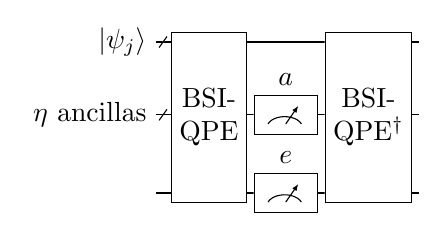
\begin{tikzpicture}
\begin{yquant*}
% init {$\eta$ ancillas} (a);
qubit {$\ket{\psi_j}$} system;
qubit {$\eta$ ancillas} a;
qubit {} f;

slash system;
slash a;
hspace {0.1cm} -;

box {BSI-\\QPE} (a,system,f);

["$a$",type=qubit]
measure a;

["$e$",type=qubit]
measure f;

box {BSI-\\QPE$^{\dagger}$} (a,system,f);
\end{yquant*}
\end{tikzpicture}

\caption{Quantum circuit for implementing projective measurement $E_{ae}$. }
\label{fig:Ecircuit}
\end{figure}
This measurement gives us $(-1)^ea$ which approximates the energy $E_a$ of the initial state. It is important to note that due to the measurement this will not return the ancilla qubits to a completely disentangled state. It is crucial that the $\eta$ ancilla register that will be used to store $a$ begin each full update process in the $\ket{0}$ state. 
\subsection{Update}
\label{section:update}
After measuring the initial energy we must apply an update to our state. In quantum metropolis this update comes in the form of a unitary operator $C$ chosen from some set $\mathcal{C}$ according to some probability measure $d\mu(C)$. It is essential for the purposes of detailed balance that the probability of choosing $C \in \mathcal{C}$ is equal to the probability of choosing $C^{\dagger} \in \mathcal{C}$ (which is alternatively expressed as $d\mu(C) = d\mu(C^{\dagger})$).
\subsection{Accept or Reject}
\label{section:acceptprob}
After applying our unitary update $C$ we must decide whether to accept or reject this update. To ensure the probability of acceptance is approximately $\tilde{f}_{E_aE_b}$, we use a combination of phase estimation, controlled rotations and single qubit measurement (illustrated in Fig~\ref{fig:Qcircuit}). First we use phase estimation to prepare an ancilla register with an approximation $b$ to the new energy $E_b$:
\begin{equation}
   \frac{1}{\sqrt{2^{\eta}}}\sum_{j,b,p}G_j^{bp}\otimes\ket{b}\bra{p}\otimes\ket{\psi_j}\bra{\psi_j}
\end{equation}
Then using the known initial energy estimate $a$ we perform a $W_{a}$ rotation upon an ancilla qubit (initialised to $\ket{0}$ at the beginning of the update process) controlled by the ancilla register (and conditioned on the measurement result $e$ from $E_{ae}$):
\begin{equation}
    W_{abde} = \begin{pmatrix}
        \sqrt{1 - f_{abde}} & \sqrt{f_{abde}}\\
       \sqrt{f_{abde}} & -\sqrt{1 - f_{abde})}
    \end{pmatrix}
\end{equation}
Therefore, upon measuring this ancilla qubit the probability of measuring $s=1$ is given by $f_{abde}$ which we choose such that it is approximately $\tilde f_{E_aE_b}$. This is insufficient to prove that quantum metropolis converges to a gibbs state, however it does highlight the similarities with classical metropolis. In Section~\ref{section:why} we will prove the convergence rigorously.

If we measure $s=0$ (reject), then we proceed by applying $W_{a}^{\dagger}$ ($=W_a$) again after the measurement before applying inverse phase estimation and $C^{\dagger}$, to make the whole sequence ($Q_s^{ae}$) a projective binary measurement:
\begin{equation} 
    Q_s^{ae} = \frac{1}{2^{\eta}}\sum_{j,p,q,b,d}  C^{\dagger}\ket{\psi_j}\bra{\psi_j}C \otimes \ket{q}\bra{p} \otimes G_j^{bq\dagger}\ket{d}\bra{d}G_j^{bp}\otimes R^{abde}_s
\end{equation}
where $R^{abde}_s = W_{abde}\ket{s}\bra{s}W_{abde}$. If instead we measure $s=1$ (accept) we simply measure the energy register and then apply inverse BSI-QPE. We represent this accept process as $L^a_b$ as defined in Fig.~\ref{fig:LQ_circuit} and gives the following operator:
\begin{equation}
    L^{ade}_b = \frac{1}{2^{\eta}}\sum_{j,p,q}\ket{\psi_j}\bra{\psi_j}C \otimes \ket{q}\bra{p} \otimes G^{bq\dagger}_j \ket{d}\bra{d}G^{bp}_j \otimes \ket{1}\bra{1}W_{abde}
\end{equation}

It is crucial that the $\eta+2$ ancillas used in this first $Q^a_s$ measurement are different to those used in the $E_a$ measurement, and begin initialized to $\ket{0}$ at the beginning of each update process. However, it is equally important that every subsequent $Q_s^a$ measurement within the same update process reuses the ancillas without resetting them. This is highlighted by Fig.~\ref{fig:fullcircuit}. If instead ancillas were reset between measurements, then the Marriott and Watrous rewinding argument presented below is invalidated.
\begin{figure}
\begin{tikzpicture}
\begin{yquant*}
% init {$\eta$ ancillas} (a);
qubit {$\ket{\psi_j}$} system;
qubit {$\eta+1$ ancillas} a;
qubit {ancilla} f;

slash system;
slash a;
hspace {0.1cm} -;
box {$C$} (system);
box {BSI-\\QPE} (a,system);
[multictrl]
box {$W_{abde}$} (f) ~ a;



["$s$",type=qubit]
measure f;
% text {$\ket{b}$} (a);


[multictrl]
box {$W_{abde}$} (f) ~ a;

box {BSI-\\QPE$^{\dagger}$} (a,system);
box {$C^{\dagger}$} (system);
\end{yquant*}
\end{tikzpicture}

\caption{Quantum circuit for implementing projective measurement $Q_s^{ae}$. The same measurement ancilla is reused in every $Q_s^{ae}$ in an update step without being reset. It is necessary to apply $W_{abde}$ before and after the measurement to make the whole measurement projective (as $W_{abde}^{\dagger} = W_{abde}$). The slashed control is used to denote multiplexed control \cite{low2024trading}.}
\label{fig:Qcircuit}
\end{figure}

\begin{figure}
\begin{tikzpicture}
\begin{yquant*}
% init {$\eta$ ancillas} (a);
qubit {$\ket{\psi_j}$} system;
qubit {$\eta+1$ ancillas} a;
qubit {ancilla $\ket{0}$} f;

slash system;
slash a;
hspace {0.1cm} -;
box {$C$} (system);
box {BSI-\\QPE} (a,system);
[multictrl]
box {$W_{abde}$} (f) ~ a;



["$s=1$",type=qubit]
measure f;
["$b\>\>d$",type=qubit]
measure a;
% text {$\ket{b}\bra{b}$} (a);
box {BSI-\\QPE$^{\dagger}$} (a,system);
\end{yquant*}
\end{tikzpicture}

\caption{Quantum circuit for implementing accept process $L_b^a$.}
\label{fig:LQ_circuit}
\end{figure}
\subsection{Rejection process}
Upon rejection in the classical algorithm we can simply revert back to an earlier copy we made of the initial state or we may be able to reverse the update applied. However, in the quantum setting the no-cloning principle rules out the former and the irreversibility of measurement rules out the latter. Therefore, we need a new technique to return to our initial state.

We use an iterative sequence of binary projective measurements similar to the QMA verification amplification of Marriott and Watrous \cite{MarriottWatrous}. The first measurement $Q_s^{ae}$ has already been introduced, whilst the second $P_s^{ae}$ simply reports whether the state has returned to the initial energy:


\begin{equation}
    P^{ae}_1 = \frac{1}{2^{\eta}}\sum_{j,p,q} \left( \ket{\psi_j}\bra{\psi_j} \otimes \ket{q}\bra{p} \otimes G_j^{aq\dagger}\ket{e}\bra{e}G_j^{ap} \right)
\end{equation}
\begin{multline}
    P^{ae}_0 = \frac{1}{2^{\eta}}\sum_{j,p,q} \sum_{b}\bigg( \ket{\psi_j}\bra{\psi_j} \otimes \ket{q}\bra{p} \otimes \\G_j^{bq\dagger}(\mathbb{I} - \delta_{ab}\ket{e}\bra{e})G_j^{bp}  \bigg)
\end{multline}
This measurement is conducted as demonstrated by Fig~\ref{fig:Pcircuit}. It is crucial that the $\eta + 1$ ancillas used in $P_s^{ae}$ are the same as those used in $E_a$, and that the same ancillas are reused in every subsequent application of $P_s^{ae}$ as shown in Fig~\ref{fig:fullcircuit}.
\begin{figure}
\begin{tikzpicture}
\begin{yquant*}
% init {$\eta$ ancillas} (a);
qubit {$\ket{\psi_j}$} system;
qubit {$\eta+1$ ancillas} a;
qubit {$\ket{0}$} f;

slash system;
slash a;
hspace {0.1cm} -;
box {BSI-QPE} (a,system);

[multictrl]
box { $X$} f ~ a;

["$s$",type=qubit]
measure f;


box {BSI-QPE$^{\dagger}$} (a,system);
\end{yquant*}
\end{tikzpicture}

\caption{Quantum circuit for implementing projective measurement $P_s^{ae}$. The measurement ancilla introduced here does not need to be reused in each $P_s^{ae}$, unlike the measurement ancilla in $Q_s^{ae}$. The controlled $X$ gate is only triggered by the state $\ket{a}\ket{e}$ on the ancilla registers.}
\label{fig:Pcircuit}
\end{figure}
\begin{figure*}
    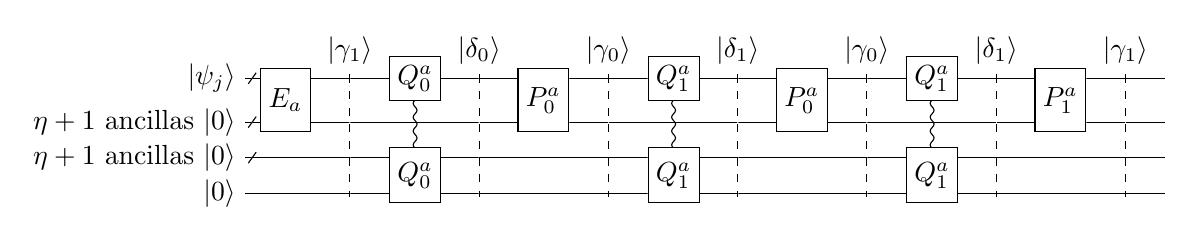
\begin{tikzpicture}
\begin{yquant*}
qubit {$\ket{\psi_j}$}  s;
qubit {$\eta +1$ ancillas $\ket{0}$} panc;
qubit {$\eta +1$ ancillas $\ket{0}$} qanc;
qubit {$\ket{0}$} m;
slash s;
slash qanc;
slash panc;
hspace {0.1cm} -;
box {$E_a$} (s,panc);
["$\ket{\gamma_1}$"]
barrier (-);
box {$Q^a_0$} (s,qanc, m);
["$\ket{\delta_0}$"]
barrier (-);
box {$P^a_0$} (s,panc);
["$\ket{\gamma_0}$"]
barrier (-);
box {$Q^a_1$} (s,qanc, m);
["$\ket{\delta_1}$"]
barrier (-);
box {$P^a_0$} (s,panc);
["$\ket{\gamma_0}$"]
barrier (-);
box {$Q^a_1$} (s,qanc, m);
["$\ket{\delta_1}$"]
barrier (-);
box {$P^a_1$} (s,panc);
["$\ket{\gamma_1}$"]
barrier (-);
\end{yquant*}
\end{tikzpicture}
\caption{Successfully completed rejection procedure demonstrating how the ancilla qubits used for $Q_s^{ae}$ are only reused by $Q_s^{ae}$ and the same for $P_s^{ae}$. This circuit corresponds to a term in $\mathcal{B}(2)[\rho]$ for $\{s_n\} = \{1,1\}$ and, within a single invariant subspace $\lambda$ (see Section~\ref{section:rejection}), occurs with probability $(1-p^{aej}_{\lambda})^4(p^{aej}_{\lambda})^2$. The state labels at the barriers denote the corresponding states of each invariant subspace.}
\label{fig:fullcircuit}
\end{figure*}

The iterative process proceeds as follows after measuring $s=0$ (reject) from the initial $Q_s^{ae}$ measurement: 
\begin{enumerate}
    \item Measure $P_s^{ae}$
        \begin{enumerate}
            \item If $s=1$ \textbf{terminate} as the state has returned to the approximate energy of the initial state.
            \item If $s=0$ continue.
        \end{enumerate}
    \item Measure $Q_s^a$
    \item Repeat up to a maximum of $n^*$ iterations
\end{enumerate}
% Each repetition has a constant chance of success as shown below and hence the iterative process has an exponentially small probability of failing to correctly reject the update, as we will now demonstrate using techniques originating in \cite{MarriottWatrous}. 

Let us consider the action of the rejection process on each eigenvector $\ket{\psi_j}$ of $H$. After measuring the energy $a$ at the beginning of the metropolis step we are left with post-measurement state $\frac{E_{ae}\ket{\psi_j}\ket{0}}{\|E_{ae} \ket{\psi_j}\ket{0}\|}$. We can see that this state must be a $+1$ eigenstate of the projector $P^{ae}_1$ due to the relation $P_1^{ae}E_{ae} = E_{ae}$.  Furthermore, as $P_1^{ae}$ commutes with $P^{ae}_1Q^{ae}_0P^{ae}_1$ they must be jointly diagnosable. Therefore our post measurement state can be written as a sum of joint eigenstates $\ket{\gamma_1^{a \lambda}}$ of $P^{ae}_1Q^{ae}_0P^{ae}_1$ and $P_1^{ae}$:
\begin{equation}
    \frac{E_{ae}\ket{\psi_j}\ket{0}}{\|E_{ae} \ket{\psi_j}\ket{0}\|} = \sum_{\lambda} c_{\lambda}^{aej}\ket{\gamma_1^{ae \lambda}}
\end{equation}
Writing the eigenvalue of $\ket{\gamma^{ae\lambda}_1}$ as $1-p^{ae\lambda}$, we have: \begin{align}1-p^{ae\lambda}&=\bra{\gamma^{ae\lambda}_1}P^{ae}_1Q^{ae}_0P^{ae}_1\ket{\gamma^{ae\lambda}_1} \\&=\|Q^{ae}_0P^{ae}_1\ket{\gamma^{aej\lambda}_1}\|^2\\ &= 1-\|Q^{ae}_1\ket{\gamma^{ae\lambda}_1}\|^2
\end{align}
so $p^{ae\lambda} = \|Q^{ae}_1\ket{\gamma^{ae\lambda}_1}\|^2$, and the probability of accepting the update is given by the mixture $p_{aej} = \sum_{\lambda}|c^{aej}_{\lambda}|^2p^{ae\lambda}$. Therefore, for each $\lambda$ with $p^{ae\lambda} \in (0,1)$ we can define the following 2D invariant subspace (we have suppressed the $ae\lambda$ labels for the remainder of this section for clarity, writing $\ket{\gamma_1} = \ket{\gamma^{ae\lambda}_1}$ and $p = p^{ae\lambda}$):
\begin{align}
    \ket{\delta_0} &= \frac{Q^{ae}_0P^{ae}_1\ket{\gamma_1}}{\sqrt{1-p}} &\ket{\delta_1} &= \frac{Q^{ae}_1P^{ae}_1\ket{\gamma_1}}{\sqrt{p}} \\
    \ket{\gamma_0} &= \frac{P^{ae}_0Q^{ae}_0\ket{\delta_0}}{\sqrt{p}} &\ket{\gamma_1} &= \frac{P^{ae}_1Q^{ae}_0\ket{\delta_0}}{\sqrt{1-p}}
\end{align}
From these definitions the following relations can be deduced:
\begin{align}
\begin{split}
\label{eq:deltagamma0}
    P^{ae}_1 \ket{\gamma_1} &= (Q^{ae}_0+Q^{ae}_1)P^{ae}_1 \ket{\gamma_1}\\
    &= Q^{ae}_0P^{ae}_1 \ket{\gamma_1}+Q^{ae}_1P^{ae}_1 \ket{\gamma_1}\\
    &= \sqrt{1-p} \ket{\delta_0} + \sqrt{p}\ket{\delta_1}\\
    Q^{ae}_0\ket{\delta_0} &= \sqrt{p} \ket{\gamma_0} + \sqrt{1-p} \ket{\gamma_1}
\end{split}
\end{align}
As $P^{ae}_1 \ket{\gamma_1} = \ket{\gamma_1}$ and $Q^{ae}_0\ket{\delta_0} = \ket{\delta_0}$ we can simplify the above and then through substitution deduce the remaining relations:
\begin{align}
\begin{split}
\label{eq:deltagamma1}
        \ket{\delta_1} &= -\sqrt{1-p} \ket{\gamma_0} + \sqrt{p} \ket{\gamma_1}\\
    \ket{\gamma_0} &= \sqrt{p} \ket{\delta_0} - \sqrt{1-p}\ket{\delta_1}
\end{split}
\end{align}
Therefore it is clear that each measurement transitions the state from one of $\ket{\delta_i}$ to one of $\ket{\gamma_i}$ or vice versa, whilst remaining within the same 2D invariant subspace. As the subspaces corresponding to different $\lambda$ are mutually orthogonal (which follows from the orthogonality of the $\ket{\gamma^{ae\lambda}_1}$ together with the relations above) and each is preserved by both measurements, the subspaces do not mix at any point during the rejection process. The probability of these transitions are trivially deduced from \eqref{eq:deltagamma0} and \eqref{eq:deltagamma1}, and can be seen in Fig.~\ref{fig:transitions}.
\begin{figure}
    \centering
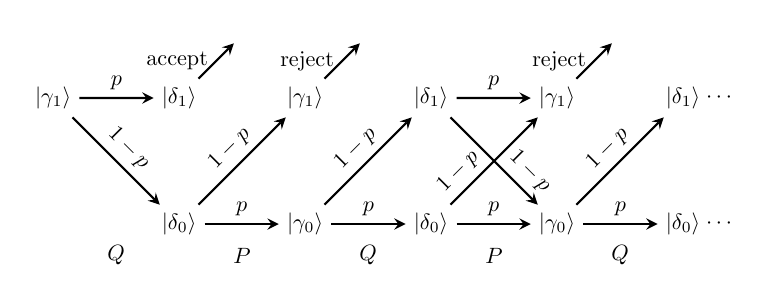
\begin{tikzpicture}[node distance=2cm, >=stealth, thick, scale=0.8, transform shape]
    \node (g-1t) at (0,2) {$|\gamma_1\rangle$};
    \node (s0t)  at (2,2) {$|\delta_1\rangle$};
    \node (s0)  at (2,0) {$|\delta_0\rangle$};
    \node (g0)  at (4,0) {$|\gamma_0\rangle$};
    \node (s1)  at (6,0) {$|\delta_0\rangle$};
    \node (g1)  at (8,0) {$|\gamma_0\rangle$};
    \node (s2)  at (10,0) {$|\delta_0\rangle$};
    \node (...1) at (10.6,0) {$\cdots$};
    \node (...2) at (10.6,2) {$\cdots$};
    
    \node (a) at (3,3) {};
    \node (r1) at (5,3) {};
    \node (r2) at (9,3) {};
    
    \node (g1t) at (4,2) {$|\gamma_1\rangle$};
    \node (s1t) at (6,2) {$|\delta_1\rangle$};
    \node (g2t) at (8,2) {$|\gamma_1\rangle$};
    \node (s2t) at (10,2) {$|\delta_1\rangle$};
    
    % Transitions
    \draw[->] (s0) -- node[above] {$p$} (g0);
    \draw[->] (g0) -- node[above] {$p$} (s1);
    \draw[->] (s1) -- node[above] {$p$} (g1);
    \draw[->] (g1) -- node[above] {$p$} (s2);
    
    \draw[->] (s0) -- node[above,sloped] {$1-p$} (g1t);
    \draw[->] (g0) -- node[above ,sloped] {$1-p$} (s1t);
    \draw[->] (s1) -- node[above left,sloped] {$1-p$} (g2t);
    \draw[->] (s1t) -- node[above] {$p$} (g2t);
    \draw[->] (g-1t) -- node[above] {$p$} (s0t);
    
    \draw[->] (s1t) -- node[above right,sloped] {$1-p$} (g1);
    \draw[->] (g1) -- node[above ,sloped] {$1-p$} (s2t);
    \draw[->] (g-1t) -- node[above ,sloped] {$1-p$} (s0);

    \draw[->] (s0t) -- node[left] {accept} (a);
    \draw[->] (g1t) -- node[left] {reject} (r1);
    \draw[->] (g2t) -- node[left] {reject} (r2);

    % Labels
    \node at (1,-0.5) {$Q$};
    \node at (3,-0.5) {$P$};
    \node at (5,-0.5) {$Q$};
    \node at (7,-0.5) {$P$};
    \node at (9,-0.5) {$Q$};
\end{tikzpicture}
    \caption{Markov chain showing the transition probability between the 4 states of a single invariant subspace $\lambda$ (with $p = p^{ae\lambda}$) upon each projective measurement. The full rejection process is a mixture of such chains weighted by $|c^{aej}_{\lambda}|^2$.}
    \label{fig:transitions}
\end{figure}

From this we can calculate the probability of attempting to reject and then failing the rejection process within a single invariant subspace to be $p(1-p)(p^2 +(1-p)^2)^{n^*}$. As the subspaces do not mix, the overall failure probability $p_a^{fail}$ is the corresponding mixture over subspaces (reinstating the suppressed labels):
\begin{equation}
   p_{ae}^{fail} =  \sum_{\lambda}|c^{aej}_{\lambda}|^2p^{ae\lambda}(1-p^{ae\lambda})((p^{ae\lambda})^2 +(1-p^{ae\lambda})^2)^{n^*}
\end{equation}
For all $p \in [0,1]$ we have: 
\begin{equation}
    p(1-p)(p^2 +(1-p)^2)^{n^*} \leq \frac{1}{2(n^*+1)} \left(\frac{n^*}{n^*+1}\right)^{n^*}
\end{equation}
Therefore, as $\sum_{\lambda}|c^{aej}_{\lambda}|^2=1$ we have:
\begin{equation}
    \label{eq:probabilty_of_rejection}
   p_{ae}^{fail} \leq \frac{1}{2(n^*+1)} \left(\frac{n^*}{n^*+1}\right)^{n^*} \leq \frac{1}{2n^*}
\end{equation}
If the rejection process fails then the whole algorithm fails irrecoverably and must be restarted from the original initial state.

% We can evaluate $p_{aj}$ exactly as:
% \begin{equation}
%     p_{aj} = \sum_{\substack{b,k,\\p,q}} f_{ab}\alpha^{aq}_j \alpha_j^{ap} \alpha_k^{bp} \alpha_k^{bq} \| \bra{\psi_j} C \ket{\psi_k}\|^2
%     \label{eq:paj_exact}
% \end{equation}
\label{section:rejection}

\section{Why it works}
\label{section:why}
The classical Metropolis-Hastings algorithm works by constructing a Markov Chain through proposing and accepting/rejecting moves with probabilities determined by the energy difference between the initial and modified states. The transition matrix of this Markov chain is in detailed balance with respect to the Gibbs state, implying that the Gibbs state is a fixed point of the Markov chain. As Markov chain is also ergodic, it is known that it must have a single unique fixed point and converge towards it. Therefore, the Markov chain converges to the Gibbs state.

In the quantum metropolis algorithm we similarly construct a quantum Markov chain by proposing and accepting/rejecting moves based upon energy differences. However, as the energy differences cannot be resolved exactly we cannot prove exact detailed balance and must propose an alternative notion of approximate quantum detailed balance. A number of different definitions of approximate quantum detailed balance are already present in the literature \cite{}, however, we must go beyond these to incorporate additive errors to fully account for the non-zero (but exponentially suppressed) tails of BSI-QPE. By showing that the CP map that characterises the quantum Markov chain is in approximate quantum detailed balance with respect to the Gibbs state we know that the fixed point of the quantum Markov chain is very close to the Gibbs state. Further, we can ensure the quantum Markov chain is ergodic by choosing our update set $\{C\}$ to be a universal gate set \cite{Temme_2011} and hence that the quantum Markov chain converges to the fixed point close to the Gibbs state.

Below we present our modified formulation of approximate quantum detailed balance:

For any completely positive map $\mathcal{M}$ ($\mathcal{M}[\rho] =\sum_{j}  A_{j}\rho  A^{\dagger}_{j}$) and density matrix $\sigma$, we define $\mathcal{M}_{\sigma}[\rho] =\sum_{j}  A_{j}\sigma^{\frac{1}{2}}\rho\sigma^{\frac{1}{2}}  A^{\dagger}_{j}$ and $ \mathcal{M}^*_{\sigma}[\rho] = \sum_{j} \sigma^{\frac{1}{2}}A^{\dagger}_{j}\rho A_{j}\sigma^{\frac{1}{2}}$.
\begin{lemma}
\label{lemma:1}
Given a completely positive map $\mathcal{M}$ on $d$-dimensional density matrices and a density matrix $\sigma$.  If for all density matrices $\rho$ and operators $X$ (such that $\|X\|=1$), we have:
\begin{equation}
    Tr\left[X \mathcal{M}^*_{\sigma}[\rho]\right] = Tr\left[X\mathcal{M}_{\sigma}[\rho]\right](1+\epsilon^{X}_m) + \epsilon^{X}_a
    \label{eq:approximate_quantum_detailed_balance_condition}
\end{equation}
where $|\epsilon^{X}_m| \leq \epsilon_m$, $|\epsilon^{X}_a| \leq \epsilon_a$, then:
 \begin{equation}
    \|\mathcal{M}^*_{\sigma}[\mathbb{I}]-\mathcal{M}[\sigma] \|_* \leq \|\mathcal{M}[\sigma]\|_*\epsilon_m + d\epsilon_a
\end{equation}
where $\|\cdot\|_*$ is trace-norm and $\|\cdot\|$ is operator-norm.
\end{lemma}

\begin{proof}
    If \eqref{eq:approximate_quantum_detailed_balance_condition} holds then for $\rho = \frac{\mathbb{I}}{d}$:
    \begin{equation}
        Tr\left[X (\mathcal{M}^*_{\sigma}[\mathbb{I}]-\mathcal{M}_{\sigma}[\mathbb{I}])\right] = Tr\left[X\mathcal{M}_{\sigma}[\mathbb{I}]\right]\epsilon^{X}_m + d\epsilon^{X}_a
    \end{equation}
    Further, by definition:
    \begin{equation}
        \mathcal{M}_{\sigma}[\mathbb{I}] = \mathcal{M}[\sigma]
    \end{equation}
    Therefore,
    \begin{equation}
    \label{eq:lhs}
        Tr\left[X (\mathcal{M}^*_{\sigma}[\mathbb{I}]-\mathcal{M}[\sigma])\right] = Tr\left[X\mathcal{M}[\sigma]\right]\epsilon^{ X}_m + d\epsilon^{X}_a
    \end{equation}
    By the H\"older inequality for Schatten norms we can see that: 
        \begin{equation}
        |Tr[X\mathcal{M}[\sigma]]| \leq \|X\|\|\mathcal{M}[\sigma]\|_*
    \end{equation}
    By taking the SVD of $(\mathcal{M}^*_{\sigma}[\mathbb{I}]-\mathcal{M}[\sigma]) = U\Sigma V^{\dagger}$ we can see that by choosing $X = VU^{\dagger}$ we have $Tr(X(\mathcal{M}^*_{\sigma}[\mathbb{I}]-\mathcal{M}[\sigma])) = \|\mathcal{M}^*_{\sigma}[\mathbb{I}]-\mathcal{M}[\sigma]\|_*$, and hence:
    \begin{equation}
        \|\mathcal{M}^*_{\sigma}[\mathbb{I}]-\mathcal{M}[\sigma]\|_* \leq \|\mathcal{M}[\sigma]\|_*\epsilon_m + d\epsilon_a
    \end{equation}
\end{proof}
\begin{theorem}[Approximate Quantum Detailed Balance]
\label{theorem:quantumapproximatedeatildedbalance}
Given a completely positive trace preserving map $\mathcal{E}$ on $d$-dimensional density matrices constructed from a sum of completely positive maps $\mathcal{M}_j$:
\begin{equation}
    \mathcal{E}[\rho] = \sum_j \mathcal{M}_j[\rho]
\end{equation}
If every $\mathcal{M}_j$ satisfies Lemma~\ref{lemma:1} for the same given density matrix $\sigma$ with respective multiplicative $\epsilon_m^j$ and additive $\epsilon_a^j$ errors. Then we have:
\begin{multline}
     \|\mathcal{E}[\sigma]-\sigma\|_* \leq \\\sum_j\min\left(\|\mathcal{M}_j[\sigma]\|_*\epsilon^j_m + d\epsilon^j_a, 2\|\mathcal{M}_j[\sigma]\|_*\right)
\end{multline}
\end{theorem}
\begin{proof}
    By the triangle inequality we have:
    \begin{equation}
        \|\mathcal{E}^*_{\sigma}[\mathbb{I}]-\mathcal{E}[\sigma]\|_* \leq \sum_j \|\mathcal{M}^*_{j\sigma}[\mathbb{I}]-\mathcal{M}_{j}[\sigma]\|_*
    \end{equation}
    As $\mathcal{E}$ is trace-preserving, we know that:
    \begin{equation}
        \mathcal{E}^*_{\sigma}[\mathbb{I}] = \sum_{j} \sigma^{\frac{1}{2}}A^{\dagger}_{j} A_{j}\sigma^{\frac{1}{2}} = \sigma
    \end{equation}
    Therefore,
    \begin{equation}
        \|\sigma - \mathcal{E}[\sigma]\|_* \leq \sum_j \|\mathcal{M}^*_{j\sigma}[\mathbb{I}]-\mathcal{M}_{j}[\sigma]\|_*
    \end{equation}
    By Lemma~\ref{lemma:1} we have that for all $j$:
    \begin{equation}
        \|\mathcal{M}^*_{j\sigma}[\mathbb{I}]-\mathcal{M}_{j}[\sigma]\|_* \leq \|\mathcal{M}_j[\sigma]\|_*\epsilon^j_m + d\epsilon^j_a
    \end{equation}
    Further, as both
$\mathcal{M}_{j,\sigma}^{*}[\mathbb{I}]$ and
$\mathcal{M}_j[\sigma]$ are positive semidefinite:
    \begin{align}
        \|\mathcal{M}^*_{j\sigma}[\mathbb{I}]\|_* &= Tr\left[\sum_l \sigma^{\frac{1}{2}} K_{jl}^{\dagger} \mathbb{I} K_{jl} \sigma^{\frac{1}{2}}\right]\\
        &= Tr\left[\sum_l K_{jl}\sigma K_{jl}^{\dagger}\right]\\
        &= \|\mathcal{M}_{j}[\sigma]\|_*
    \end{align}
    Therefore,
    \begin{equation}
         \|\mathcal{M}^*_{j\sigma}[\mathbb{I}]-\mathcal{M}_{j}[\sigma]\|_* \leq 2\|\mathcal{M}_{j}[\sigma]\|_*
    \end{equation}
    Hence,
    \begin{multline}
        \|\sigma-\mathcal{E}[\sigma]\|_* \leq \\\sum_j \min \left(\|\mathcal{M}_j[\sigma]\|_*\epsilon^j_m + d\epsilon^j_a, 2\|\mathcal{M}_{j}[\sigma]\|_*\right)
    \end{multline}
\end{proof}
% \begin{theorem}[Approximate Quantum Detailed Balance]
% \label{theorem:quantumapproximatedeatildedbalance}
%     Given a completely positive trace preserving
% map $\mathcal{E}$ on $d$-dimensional density matrices and a density matrix $\sigma$. Let $\mathcal{E}[\rho] =\sum_{j}  A_{j}\rho  A^{\dagger}_{j}$, $\mathcal{E}_{\sigma}[\rho] =\sum_{j}  A_{j}\sigma^{\frac{1}{2}}\rho\sigma^{\frac{1}{2}}  A^{\dagger}_{j}$ and $ \mathcal{E}^*_{\sigma}[\rho] = \sum_{j} \sigma^{\frac{1}{2}}A^{\dagger}_{j}\rho A_{j}\sigma^{\frac{1}{2}}$. If for all density matrices $\rho$ and operators $X$ with operator norm 1, we have:
% \begin{equation}
%     Tr\left[X \mathcal{E}_{\sigma}[\rho]\right] = Tr\left[X\mathcal{E}^*_{\sigma}[\rho]\right](1+\epsilon^{\rho \Pi}_m) + \epsilon^{\rho \Pi}_a
%     \label{eq:approximate_quantum_detailed_balance_condition}
% \end{equation}
% where $|\epsilon^{\rho \Pi}_m| \leq \epsilon_m$, $|\epsilon^{\rho \Pi}_a| \leq \epsilon_a$, then $\mathcal{E}$ is said to obey Approximate Quantum Detailed Balance with respect to $\sigma$. Therefore,
%  \begin{equation}
%     \|\mathcal{E}[\sigma] - \sigma\|_* \leq \epsilon_m + d\epsilon_a
% \end{equation}
% where $\|\cdot\|_*$ is the trace norm.
% \end{theorem}
% \begin{proof}
%     If \eqref{eq:approximate_quantum_detailed_balance_condition} holds then for $\rho = \frac{\mathbb{I}}{d}$:
%     \begin{equation}
%         Tr\left[X (\mathcal{E}_{\sigma}[\mathbb{I}]-\mathcal{E}^*_{\sigma}[\mathbb{I}])\right] = Tr\left[X\mathcal{E}^*_{\sigma}[\mathbb{I}]\right]\epsilon^{X}_m + d\epsilon^{X}_a
%     \end{equation}
%     Further, by definition:
%     \begin{equation}
%         \mathcal{E}^*_{\sigma}[\mathbb{I}] = \sum_{j} \sigma^{\frac{1}{2}}A^{\dagger}_{j} A_{j}\sigma^{\frac{1}{2}} = \sigma
%     \end{equation}
%     \begin{equation}
%         \mathcal{E}_{\sigma}[\mathbb{I}] = \mathcal{E}[\sigma]
%     \end{equation}
%     Therefore,
%     \begin{equation}
%         Tr\left[X (\mathcal{E}[\sigma]-\sigma)\right] = Tr\left[X\sigma\right]\epsilon^{ X}_m + d\epsilon^{X}_a
%     \end{equation}
%     As $Tr\left[X\sigma\right] \leq 1$ and $\|A\|_* = \max_{\|X\|=1} |Tr(XA)|$ we have that:
%     \begin{equation}
%         \|\mathcal{E}[\sigma]-\sigma\|_* \leq \epsilon_m + d\epsilon_a
%     \end{equation}
% \end{proof}
%  \begin{corollary}[Ergodicity of the square modulus for random-unitary channels \cite{Burgarth_2013}]
%      A random-unitary channel $M = \sum_{i\in X}p_i \mathcal{U}_i$ , with $\mathcal{U}_i (\rho) = U_i \rho U^{\dagger}_i$ , is mixing if the group representation
% generated by the unitaries $\{U^{\dagger}_i U_j \}_{i,j\in X}$ is irreducible. 
%  \end{corollary}
\begin{widetext}
To demonstrate an update round $\mathcal{E}$ of the Quantum Metropolis algorithm is in approximate quantum detailed balance with respect to the Gibbs state $\sigma_G$, we must express it as a completely positive trace preserving map:
\begin{equation}
    \mathcal{E}[\rho] = \mathcal{A}[\rho] + \sum_{n=0}^{n^*} \mathcal{B}(n)[\rho] + \mathcal{C}[\rho]
\end{equation}
where $\mathcal{A}$ corresponding to acceptance, $\mathcal{B}(n)$ to successful rejection after $n$ iterations and $\mathcal{C}$ to failing to reject after $n^*$ iterations:
\begin{equation}
    \mathcal{A}[\rho] = \int  Tr\bigg[\sum_{a,b,d,e}L_b^{ade} E_{ae} ( \rho\otimes \ket{0}\bra{0}) 
     E_{ae}L^{ade\dagger}_b\bigg]d\mu(C)
\end{equation}
\begin{equation}
    \mathcal{B}(n)[\rho] = \int Tr\bigg[\sum_{a,e,\{s\}}P^{ae}_1Q^{ae}_{s_n}\ldots P^{ae}_0Q^{ae}_{s_1}P^{ae}_0Q^{ae}_0E_{ae} ( \rho\otimes \ket{0}\bra{0})E_{ae}Q^{ae}_0P^{ae}_0Q^{ae}_{s_1}P^{ae}_0\ldots Q^{ae}_{s_n}P^{ae}_1\bigg]d\mu(C)
\end{equation}
\begin{equation}
    \mathcal{C}[\rho] = \rho_0 \int Tr\bigg[\sum_{a,e,\{s\}}P^{ae}_0Q^{ae}_{s_{n^*}}\ldots P^{ae}_0Q^{ae}_{s_1}P^{ae}_0Q^{ae}_0E_{ae} ( \rho\otimes \ket{0}\bra{0})E_{ae}Q^{ae}_0P^{ae}_0Q^{ae}_{s_1}P^{ae}_0\ldots Q^{ae}_{s_{n^*}}P^{ae}_0\bigg]d\mu(C) 
\end{equation}
where $\rho_0$ is the initial state the overall Metropolis algorithm was started from. 


To use Theorem~\ref{theorem:quantumapproximatedeatildedbalance}, we must first evaluate Lemma~\ref{lemma:1} for $\mathcal{A}$ and $\mathcal{B}(n)[\rho]$ with respect to $\sigma_G$. To do so we will consider approximations to $\mathcal{A}$ and $\mathcal{B}(n)$ in which we have substituted $\tilde \alpha, \tilde \beta$ for $\hat \alpha, \hat \beta$. Under this substitution $G^{pq}_j$ becomes $\tilde G^{pq}_j$ such that $\|\tilde G^{pq}_j\| =0$ for all $|p-q-\frac{2^{\eta}}{2\pi}E_j|_{2^{\eta}} > \mu$. Then using Lemma~\ref{lemma:3} we will show that $\|\tilde{\mathcal{A}}-\mathcal{A}\|_* \leq \epsilon$ and $\|\tilde{\mathcal{B}}(n)-\mathcal{B}(n)\|_* \leq \epsilon$, and hence we can evaluate Lemma~\ref{lemma:1} for $\mathcal{A}$ and $\mathcal{B}(n)$. We will not evaluate Lemma~\ref{lemma:1} for $\mathcal{C}$, but rather bound its contribution in Theorem~\ref{theorem:quantumapproximatedeatildedbalance} by its trace-norm. We begin with $\tilde{\mathcal{A}}$
    \begin{equation}
    Tr\left[X\tilde{\mathcal{A}}_{\sigma_G}[\rho]\right] = \int Tr\left[(X\otimes \mathbb{I})\sum_{a,b,d,e}\textcolor{blue}{\tilde L^{ade}_b} \textcolor{red}{\tilde E_{ae}} \sigma_G^{\frac{1}{2}} (\rho\otimes \ket{0}\bra{0}) \sigma_G^{\frac{1}{2}}\textcolor{red}{\tilde E_{ae}}\textcolor{blue}{\tilde L^{ade\dagger}_b}\right] d\mu(C)
\end{equation}
As $\sigma_G = \frac{1}{Z}\sum_j e^{-\beta E_j} \ket{\psi_j}\bra{\psi_j}$ where $\ket{\psi_j}$ are the eigenstates of $H$ with eigenvalues $E_j$. 
\begin{multline}
    Tr\left[X\tilde{\mathcal{A}}_{\sigma_G}[\rho]\right] =\frac{1}{2^{4\eta}Z} \sum_{jklmabde} e^{-\frac{\beta}{2}(E_j+E_k)}\textcolor{blue}{f_{abde}} \textcolor{blue}{\bra{\psi_l}}X\textcolor{blue}{\ket{\psi_m}}\textcolor{red}{\bra{\psi_j}}\rho\textcolor{red}{\ket{\psi_k}} \int \textcolor{blue}{\braket{\psi_m|C|\psi_j}\braket{\psi_k|C^{\dagger}|\psi_l}} d\mu(C)\\\sum_{p_1p_2} \textcolor{blue}{\bra{0} \tilde G^{b0\dagger}_l\ket{d}\bra{d}\tilde G^{bp_2}_l\tilde G^{bp_2\dagger}_m\ket{d}\bra{d}\tilde G^{b0}_m\ket{0}}
    \textcolor{red}{\bra{0}\tilde G_k^{a0\dagger}\ket{e}\bra{e}\tilde G_k^{ap_1}\tilde G_j^{ap_1\dagger}\ket{e}\bra{e}\tilde G_j^{a0}\ket{0}}
    \label{eq:Arho}
\end{multline}
Similarly,
\begin{multline}
    Tr\left[X\mathcal{A}^*_{\sigma_G}[\rho]\right] =\frac{1}{2^{4\eta}Z} \sum_{jklmabde} e^{-\frac{\beta}{2}(E_l+E_m)}\textcolor{blue}{f_{abde}} \textcolor{red}{\bra{\psi_l}}X\textcolor{red}{\ket{\psi_m}}\textcolor{blue}{\bra{\psi_j}}\rho\textcolor{blue}{\ket{\psi_k}} \int \textcolor{blue}{\braket{\psi_k|C|\psi_l}\braket{\psi_m|C^{\dagger}|\psi_j}} d\mu(C)\\\sum_{p_1p_2} \textcolor{blue}{\bra{0} \tilde G^{b0\dagger}_j\ket{d}\bra{d}\tilde G^{bp_2}_j\tilde G^{bp_2\dagger}_k\ket{d}\bra{d}\tilde G^{b0}_k\ket{0}}
    \textcolor{red}{\bra{0}\tilde G_m^{a0\dagger}\ket{e}\bra{e}\tilde G_m^{ap_1}\tilde G_l^{ap_1\dagger}\ket{e}\bra{e}\tilde G_l^{a0}\ket{0}}
        \label{eq:A*rho}  
\end{multline}
Due to the restricted support of $\tilde G^{pq}_j$ we can restrict the summations in Eq.~\eqref{eq:Arho} and Eq~\eqref{eq:A*rho} to $\chi$, where $\chi$ is the set of all $a,b,d,e$ such that all of the following conditions hold:
\begin{equation}
\begin{aligned}
    |a-(-1)^e\frac{2^{\eta}}{2\pi}E_lt|_{2^{\eta}} &\leq \mu  &|a-(-1)^e\frac{2^{\eta}}{2\pi}E_mt|_{2^{\eta}} &\leq \mu\\
    |b-(-1)^{d}\frac{2^{\eta}}{2\pi}E_jt|_{2^{\eta}} &\leq \mu   &|b-(-1)^{d}\frac{2^{\eta}}{2\pi}E_kt|_{2^{\eta}}& \leq \mu
\end{aligned}
\end{equation}
 We can relax these conditions to define $\chi' \supset \chi$  as all $a,b, d, e$ such that:
\begin{equation}
\label{eq:condJ}
        |(-1)^db-(-1)^ea -\frac{2^{\eta}t}{2\pi}(\frac{E_j+E_k-E_l-E_m}{2})|_{2^{\eta}} \leq 4\mu
\end{equation}
As $|E_j| \leq \|H\|$, if we choose $t = \frac{1}{16\|H\|}$ and $\mu < \frac{2^{\eta}}{64\pi}$ so that $E_j$ satisfies $-\frac{1}{8t} + 2\frac{2\pi}{2^{\eta}t}\mu < E_j < \frac{1}{8t} - 2\frac{2\pi}{2^{\eta}t}\mu$, then we have that $-2^{\eta-2}+4\mu < \frac{2^{\eta}t}{2\pi}(E_i -E_j) < 2^{\eta-2}-4\mu$ for all $i$ and $j$. Hence, we can restrict the ranges of $(-1)^db-(-1)^ea$ found within $\chi'^C$ to the following:
\begin{multline}
    -2^{\eta+1}\leq(-1)^db-(-1)^ea<-7\cdot2^{\eta-2} \text{ or } -5\cdot2^{\eta-2}< (-1)^db-(-1)^ea < -3\cdot2^{\eta-2} \text{ or }-2^{\eta-2}< (-1)^db-(-1)^ea < 2^{\eta-2}\\ \text{ or } 3\cdot2^{\eta-2}< (-1)^db-(-1)^ea < 5\cdot2^{\eta-2}\text{ or } 7\cdot2^{\eta-2}< (-1)^db-(-1)^ea \leq 2^{\eta+1}
\end{multline}
By separately considering each of these regions we can rewrite condition~\eqref{eq:condJ} as the following:
\begin{equation}
    a,b,d,e \in \chi' \iff \begin{cases}
    |(-1)^db-(-1)^ea+2^{\eta+1}-\frac{2^{\eta}t}{2\pi}\frac{E_j+E_k-E_l-E_m}{2}|\leq 4\mu&\text{ for }-2^{\eta+1}\leq(-1)^db-(-1)^ea<-7\cdot2^{\eta-2}\\
    |(-1)^db-(-1)^ea+2^{\eta}-\frac{2^{\eta}t}{2\pi}\frac{E_j+E_k-E_l-E_m}{2}|\leq 4\mu&\text{ for }-5\cdot 2^{\eta-2}< (-1)^db-(-1)^ea < -3\cdot2^{\eta-2}\\
     |(-1)^db-(-1)^ea-\frac{2^{\eta}t}{2\pi}\frac{E_j+E_k-E_l-E_m}{2}|\leq 4\mu&\text{ for }-2^{\eta-2}< (-1)^db-(-1)^ea < 2^{\eta-2}\\
     |(-1)^db-(-1)^ea-2^{\eta}-\frac{2^{\eta}t}{2\pi}\frac{E_j+E_k-E_l-E_m}{2}|\leq 4\mu&\text{ for }3\cdot 2^{\eta-2}< (-1)^db-(-1)^ea < 5\cdot 2^{\eta-2}\\
     |(-1)^db-(-1)^ea-2^{\eta+1}-\frac{2^{\eta}t}{2\pi}\frac{E_j+E_k-E_l-E_m}{2}|\leq 4\mu&\text{ for }7\cdot2^{\eta-2}< (-1)^db-(-1)^ea \leq 2^{\eta+1}
    \end{cases}
    \label{eq:conditions}
\end{equation}
as $|x|_N = |x - kN| \text{ for } -\frac{N}{2} + kN \leq x \leq \frac{N}{2} + kN$.
Therefore, we chose $f_{abde}$ to be defined as:
\begin{equation}
    f_{abde} = \begin{cases}
    \min(1,e^{-\beta\frac{2\pi}{2^{\eta}t}((-1)^db-(-1)^ea+2^{\eta+1})})&\text{ for }-2^{\eta+1}\leq (-1)^db-(-1)^ea < -7\cdot2^{\eta-2}\\
    0&\text{ for }-7\cdot2^{\eta-2}\leq (-1)^db-(-1)^ea \leq -5\cdot2^{\eta-2}\\
    \min(1,e^{-\beta\frac{2\pi}{2^{\eta}t}((-1)^db-(-1)^ea+2^{\eta})})&\text{ for }-5\cdot 2^{\eta}< (-1)^db-(-1)^ea < -3\cdot2^{\eta-2}\\
    0&\text{ for }-3\cdot2^{\eta-2}\leq (-1)^db-(-1)^ea \leq -2^{\eta-2}\\
     \min(1,e^{-\beta\frac{2\pi}{2^{\eta}t}((-1)^db-(-1)^ea)})&\text{ for }-2^{\eta-2}<(-1)^db-(-1)^ea < 2^{\eta-2}\\
    0&\text{ for }2^{\eta-2}\leq (-1)^db-(-1)^ea \leq 3\cdot2^{\eta-2}\\
     \min(1,e^{-\beta\frac{2\pi}{2^{\eta}t}((-1)^db-(-1)^ea-2^{\eta})})&\text{ for }3\cdot 2^{\eta-2}< (-1)^db-(-1)^ea < 5\cdot2^{\eta-2}\\
     0&\text{ for }5\cdot2^{\eta-2}\leq (-1)^db-(-1)^ea \leq 7\cdot2^{\eta-2}\\
     \min(1,e^{-\beta\frac{2\pi}{2^{\eta}t}((-1)^db-(-1)^ea-2^{\eta+1})})&\text{ for }7\cdot 2^{\eta-2}< (-1)^db-(-1)^ea \leq 2^{\eta+1}
    \end{cases}
\end{equation}
so that $e^{-\frac{\beta}{2}(E_l+E_m)}f_{baed}$ for $b, a, e, d \in \chi'$ obeys:
\begin{equation}
    \begin{aligned}
    e^{-\frac{\beta}{2}(E_l+E_m)}f_{baed} &= e^{-\frac{\beta}{2}(E_l+E_m)}\min(1,e^{-\frac{\beta}{2}(E_j+E_k-E_l-E_m + 2\xi)})\\
    &= \min(e^{-\frac{\beta}{2}(E_l+E_m)}, e^{-\frac{\beta}{2}(E_j+E_k + 2\xi)})\\
    &= e^{-\frac{\beta}{2}(E_j+E_k + 2\xi)} \min(e^{-\frac{\beta}{2}(E_l+E_m-E_j-E_k-2\xi)},1)\\
    &= e^{-\frac{\beta}{2}(E_j+E_k + 2\xi)}f_{abde}\\
    &= e^{-\frac{\beta}{2}(E_j+E_k)}f_{abde}(1+O(\beta\xi))
\end{aligned}
\label{eq:fabtofba}
\end{equation}
where $|\xi| \leq \frac{8\pi}{2^{\eta}t}\mu$. Therefore, as $\chi'$ a super-set of $\chi$ we can happily restrict the summation to one over $\chi'$ and hence:
\begin{multline}
   Tr\left[X\tilde{\mathcal{A}}^*_{\sigma_G}[\rho]\right] =\frac{1}{2^{4\eta}Z} \sum_{abde\in \chi'}\sum_{jklm} e^{-\frac{\beta}{2}(E_l+E_m)}f_{abde} \bra{\psi_l}X\ket{\psi_m}\bra{\psi_j}\rho\ket{\psi_k} \int \braket{\psi_k|C|\psi_l}\braket{\psi_m|C^{\dagger}|\psi_j} d\mu(C)\\\sum_{p_1p_2} \bra{0} \tilde G^{b0\dagger}_j\ket{d}\bra{d}\tilde G^{bp_2}_j\tilde G^{bp_2\dagger}_k\ket{d}\bra{d}\tilde G^{b0}_k\ket{0}
    \bra{0}\tilde G_m^{a0\dagger}\ket{e}\bra{e}\tilde G_m^{ap_1}\tilde G_l^{ap_1\dagger}\ket{e}\bra{e}\tilde G_l^{a0}\ket{0}
\end{multline}
By swapping the labels $a \leftrightarrow b$, $d \leftrightarrow e$, $p_1 \leftrightarrow p_2$ we get:
\begin{multline}
    Tr\left[X\tilde{\mathcal{A}}^*_{\sigma_G}[\rho]\right] =\frac{1}{2^{4\eta}Z} \sum_{abde\in \chi'^C}\sum_{jklm} e^{-\frac{\beta}{2}(E_l+E_m)}f_{baed} \bra{\psi_l}X\ket{\psi_m}\bra{\psi_j}\rho\ket{\psi_k} \int \braket{\psi_k|C|\psi_l}\braket{\psi_m|C^{\dagger}|\psi_j} d\mu(C)\\\sum_{p_1p_2} \bra{0} \tilde G^{a0\dagger}_j\ket{e}\bra{e}\tilde G^{ap_1}_j\tilde G^{ap_1\dagger}_k\ket{e}\bra{e}\tilde G^{a0}_k\ket{0}
    \bra{0}\tilde G_m^{b0\dagger}\ket{d}\bra{d}\tilde G_m^{bp_2}\tilde G_l^{bp_2\dagger}\ket{d}\bra{d}\tilde G_l^{b0}\ket{0}
\end{multline}
By applying \eqref{eq:fabtofba} we get:
\begin{multline}
    Tr\left[X\tilde{\mathcal{A}}^*_{\sigma_G}[\rho]\right] =\frac{1}{2^{4\eta}Z} \sum_{abde\in \chi'^C}\sum_{jklm} e^{-\frac{\beta}{2}(E_j+E_k)}f_{abde} \bra{\psi_l}X\ket{\psi_m}\bra{\psi_j}\rho\ket{\psi_k} \int \braket{\psi_k|C|\psi_l}\braket{\psi_m|C^{\dagger}|\psi_j} d\mu(C)\\\sum_{p_1p_2} \bra{0} \tilde G^{a0\dagger}_j\ket{e}\bra{e}\tilde G^{ap_1}_j\tilde G^{ap_1\dagger}_k\ket{e}\bra{e}\tilde G^{a0}_k\ket{0}
    \bra{0}\tilde G_m^{b0\dagger}\ket{d}\bra{d}\tilde G_m^{bp_2}\tilde G_l^{bp_2\dagger}\ket{d}\bra{d}\tilde G_l^{b0}\ket{0}(1+O(\beta\xi))
\end{multline}
As $\tilde \alpha$ and $\tilde \beta$ are real we have $\bra{0} \tilde G^{a0\dagger}_j\ket{e}\bra{e}\tilde G^{ap_1}_j\tilde G^{ap_1\dagger}_k\ket{e}\bra{e}\tilde G^{a0}_k\ket{0} = \bra{0} \tilde G^{a0\dagger}_k\ket{e}\bra{e}\tilde G^{ap_1}_k\tilde G^{ap_1\dagger}_j\ket{e}\bra{e}\tilde G^{a0}_j\ket{0}$ for $j,k$ and $l,m$.
Therefore:
\begin{multline}
Tr\left[X\tilde{\mathcal{A}}^*_{\sigma_G}[\rho]\right] =\frac{1}{2^{4\eta}Z} \sum_{abde\in \chi'^C}\sum_{jklm} e^{-\frac{\beta}{2}(E_j+E_k)}f_{abde} \bra{\psi_l}X\ket{\psi_m}\bra{\psi_j}\rho\ket{\psi_k} \int \braket{\psi_k|C|\psi_l}\braket{\psi_m|C^{\dagger}|\psi_j} d\mu(C)\\\sum_{p_1p_2} \bra{0} \tilde G^{a0\dagger}_k\ket{e}\bra{e}\tilde G^{ap_1}_k\tilde G^{ap_1\dagger}_j\ket{e}\bra{e}\tilde G^{a0}_j\ket{0}
    \bra{0}\tilde G_l^{b0\dagger}\ket{d}\bra{d}\tilde G_l^{bp_2}\tilde G_m^{bp_2\dagger}\ket{d}\bra{d}\tilde G_m^{b0}\ket{0}(1+O(\beta\xi))
\end{multline}
Finally, we require that $d\mu(C) = d\mu(C^{\dagger})$ so:
\begin{equation}
    \int  \bra{\psi_k}C\ket{\psi_{l}}\bra{\psi_m}C^{\dagger} \ket{\psi_j} d\mu(C) = \int  \bra{\psi_k}C^{\dagger}\ket{\psi_{l}}\bra{\psi_m}C \ket{\psi_j} d\mu(C)
\end{equation}
Therefore, we have that:
\begin{equation}
    Tr\left[X\tilde{\mathcal{A}}^*_{\sigma_G}[\rho]\right] = Tr\left[X\tilde{\mathcal{A}}_{\sigma_G}[\rho]\right](1+O(\beta\xi))
\end{equation}

\begin{lemma}
\label{lemma:3}
Let $\{D_s\}_{s\in S}$ be mutually orthogonal projectors satisfying $\sum_{s\in S} D_s \leq \mathbb{I}$. Given a unitary $U$ define the projective measurement $K_s = U^{\dagger}D_s U$ and CP map $\mathcal{K}[\rho] = \sum_{s \in S} K_s\rho K_s^{\dagger}$. Further, given operator $\tilde U$, we define approximate measurements $\tilde K_s = \tilde U^{\dagger}D_s \tilde U$ and approximate map $\tilde{\mathcal{K}}[\rho] = \sum_{s \in S} \tilde K_s\rho \tilde K_s^{\dagger}$. If $\|U-\tilde U\| \leq \epsilon$ then 
\begin{equation}
    \|\mathcal{K} - \tilde{\mathcal{K}}\|_{\diamond} \leq 6\epsilon
\end{equation}
\end{lemma}
\begin{proof}
First, consider:
\begin{align}
    \mathcal{K}[\rho] - \tilde{\mathcal{K}}[\rho] &= \sum_{s \in S} K_s\rho K_s^{\dagger} - \tilde K_s\rho \tilde K_s^{\dagger} \\
    &= \sum_{s \in S} (K_s-\tilde K_s)\rho K_s^{\dagger} +\tilde K_s\rho (K_s^{\dagger}- \tilde K_s^{\dagger}) \label{eq:ksUdiff}
\end{align}
We have $\Phi_{R_1,R_2}[\rho] = Tr_R[R_{1}\rho R_{2}^{\dagger}]$ we have $\|\Phi_{R_1,R_2}\|_{\diamond} \leq \|R_1\| \|R_2\|$. We can use Steinspring dilation to rewrite $\eqref{eq:ksUdiff}$ as:
\begin{equation}
    \mathcal{K}[\rho] - \tilde{\mathcal{K}}[\rho] = Tr_S\left[\sum_{s\in S}\ket{s}\bra{s}\otimes(K_s-\tilde K_s)\rho K_s^{\dagger} +\sum_{s\in S}\ket{s}\bra{s}\otimes \tilde K_s\rho (K_s^{\dagger}- \tilde K_s^{\dagger})\right]
\end{equation}
Hence, we have that:
\begin{equation}
    \|\mathcal{K} - \tilde{\mathcal{K}}\|_{\diamond} \leq \left\|\sum_{s\in S}\ket{s}\bra{s}\otimes(K_s-\tilde K_s)\right\|\left(\left\|\sum_{s\in S}\ket{s}\bra{s}\otimes K_s \right\|+\left\|\sum_{s\in S}\ket{s}\bra{s}\otimes \tilde K_s \right\|\right)
\end{equation}
Let us evaluate the terms in this expression. As $U$ is unitary we have $(\sum_{s\in S}\ket{s}\bra{s}\otimes K_s^{\dagger}) (\sum_{s\in S}\ket{s}\bra{s}\otimes K_s) = \mathbb{I}$, and thus $\left\|\sum_{s\in S}\ket{s}\bra{s}\otimes K_s \right\| = 1$. Whereas for $\tilde U$ we have:
\begin{align}
    \left\|\left(\sum_{s\in S}\ket{s}\bra{s}\otimes \tilde K_s^{\dagger} \right)\left(\sum_{s\in S}\ket{s}\bra{s}\otimes \tilde K_s \right)\right\| &= \left\|\sum_{s\in S} \ket{s}\bra{s}\otimes\tilde U^{\dagger} D_s \tilde U\tilde U^{\dagger}  D_s \tilde U\right\| \\
     &\leq \|\tilde U\|^2\left\|\sum_{s\in S} \ket{s}\bra{s}\otimes\tilde U^{\dagger} D_s  \tilde U\right\|\\
     &\leq \|\tilde U\|^2 \|\tilde U^{\dagger}  \tilde U\|= \|\tilde U\|^4\\
\end{align}
Hence we have $\left\|\sum_{s\in S}\ket{s}\bra{s}\otimes \tilde K_s \right\| \leq \|\tilde U\|^2 \leq (1+\epsilon)^2$. Finally let us consider $\left\|\sum_{s\in S}\ket{s}\bra{s}\otimes[K_s(U)-K_s(\tilde U)]\right\|$.
\begin{align}
    \left\|\sum_{s\in S}\ket{s}\bra{s}\otimes(K_s-\tilde K_s)\right\| &= \left\|\sum_{s\in S}\ket{s}\bra{s}\otimes( U^{\dagger}  D_s U-\tilde U^{\dagger}  D_s \tilde U)\right\|\\
    &= \left\|\sum_{s\in S}\ket{s}\bra{s}\otimes[ (U-\tilde U)^{\dagger}  D_s U+\tilde U^{\dagger}  D_s (U-\tilde U)]\right\|\\
    &\leq \left\|\sum_{s\in S}\ket{s}\bra{s}\otimes (U-\tilde U)^{\dagger}  D_s U\right\|+\left\|\sum_{s\in S}\ket{s}\bra{s}\otimes\tilde U^{\dagger}  D_s (U-\tilde U)\right\|
\end{align}
We again consider each of these independently. As we have:
\begin{align}
   \left\| \left(\sum_{s\in S}\ket{s}\bra{s}\otimes (U-\tilde U)^{\dagger}  D_s U\right)^{\dagger} \left(\sum_{s\in S}\ket{s}\bra{s}\otimes (U-\tilde U)^{\dagger}  D_s U\right)\right\| &= \left\|\sum_{s\in S}\ket{s}\bra{s}\otimes U^{\dagger}D_s (U-\tilde U)(U-\tilde U)^{\dagger}D_s U\right\|\\
    & \leq \epsilon^2\left\|\sum_{s\in S}\ket{s}\bra{s}\otimes U^{\dagger}D_s U\right\|\\
    & \leq \epsilon^2 \|U\|^2 =\epsilon^2  
\end{align}
Hence $\left\|\sum_{s\in S}\ket{s}\bra{s}\otimes (U-\tilde U)^{\dagger}  D_s U\right\| \leq \epsilon $ and similarly $\left\|\sum_{s\in S}\ket{s}\bra{s}\otimes\tilde U^{\dagger}  D_s (U-\tilde U)\right\| \leq \epsilon (1+\epsilon)$. Therefore, we have that $\left\|\sum_{s\in S}\ket{s}\bra{s}\otimes(K_s-\tilde K_s)\right\| \leq \epsilon + \epsilon(1+\epsilon)$. Therefore,
\begin{equation}
    \|\mathcal{K} - \tilde{\mathcal{K}}\|_{\diamond} \leq \epsilon(2+\epsilon)(1+(1+\epsilon)^2)
\end{equation}
Therefore, if $\epsilon < \frac{1}{4}$, we have $\|\mathcal{K} - \tilde {\mathcal{K}}\|_{\diamond} \leq 6\epsilon$.
\end{proof}
We can see that $\mathfrak{E}[\rho] = \sum_{a,e} E_{ae} \rho E_{ae}$,$\mathcal{P}_S[\rho] = \sum_{s\in S} P_s \rho P_s$, $\mathcal{Q}_S[\rho] = \sum_{s\in S} Q_s \rho Q_s$, $\mathcal{L}[\rho] = \sum_{bd} L_{bd} \rho L^{\dagger}_{bd}$ are all CP maps of the form described in Lemma~\ref{lemma:3}. Here we have dropped the $ae$ superscript from $P_s, Q_s, L_{bd}$ by postponing the measurement of these until the end of the circuit by storing the information additional ancilla registers and controlling $P_s$, $Q_s$ and $L_{bd}$ off these ancillas. This is not necessary in practice as these are mathematically equivalent treatments, so this is simply a proof technique. Further, by Lemma~\ref{lemma:0} we have that substituting $\tilde G^{pq}_j$ for $G^{pq}_j$ produces a modified operator $\widetilde{\text{BSI-QPE}}$ such that $\|\widetilde{\text{BSI-QPE}}- \text{BSI-QPE}\| \leq \frac{\epsilon_{\Delta}}{\sqrt{2^{\eta}}}$. Therefore, we can apply Lemma~\ref{lemma:3} to $\mathfrak{E}$ and $\mathcal{P}_S$ by taking $U$ and $\tilde U$ to be BSI-QPE and $\widetilde{\text{BSI-QPE}}$. We can also trivially extend this to $\mathcal{Q}_S$ and $\mathcal{L}_S$ as $C$ and $W_{abde}$ remain unmodified. Therefore, we have:
\begin{equation}
    \|\mathfrak{E} - \tilde{\mathfrak{E}}\|_{\diamond} \leq \frac{6\epsilon_{\Delta}}{\sqrt{2^{\eta}}} \qquad\|\mathcal{P}_S - \tilde{\mathcal{P}}_S\|_{\diamond} \leq \frac{6\epsilon_{\Delta}}{\sqrt{2^{\eta}}} \qquad\|\mathcal{Q}_S - \tilde{\mathcal{Q}}_S\|_{\diamond} \leq \frac{6\epsilon_{\Delta}}{\sqrt{2^{\eta}}}  \qquad\|\mathcal{L} - \tilde{\mathcal{L}}\|_{\diamond} \leq \frac{6\epsilon_{\Delta}}{\sqrt{2^{\eta}}} 
\end{equation}
Further, we can write $\mathcal{A}$ and $\tilde{\mathcal{A}}$ as:
\begin{equation}
    \mathcal{A}[\rho] = \mathcal{L} \circ \mathfrak{E} [\rho] \qquad  \tilde{\mathcal{A}}[\rho] = \tilde{\mathcal{L}} \circ \tilde{\mathfrak{E}} [\rho]
\end{equation}
Therefore, we can write:
\begin{align}
    \|\mathcal{A} - \tilde{\mathcal{A}}\|_{\diamond} &= \|\mathcal{L} \circ \mathfrak{E} - \tilde{\mathcal{L}} \circ \tilde{\mathfrak{E}}\|_{\diamond}\\
    &=\|(\mathcal{L}-\tilde{\mathcal{L}}) \circ \mathfrak{E} + \tilde{\mathcal{L}} \circ (\mathfrak{E}-\tilde{\mathfrak{E}})\|_{\diamond}\\
    &\leq\|\mathcal{L}-\tilde{\mathcal{L}}\|_{\diamond} \|\mathfrak{E} \|_{\diamond}+ \|\tilde{\mathcal{L}}\|_{\diamond} \|\mathfrak{E}-\tilde{\mathfrak{E}}\|_{\diamond}\\
    &\leq \frac{6\epsilon_{\Delta}}{\sqrt{2^{\eta}}}(1+\|\tilde{\mathcal{L}}\|_{\diamond})\\
    &\leq \frac{6\epsilon_{\Delta}}{\sqrt{2^{\eta}}}(2+\frac{6\epsilon_{\Delta}}{\sqrt{2^{\eta}}})
\end{align}
Therefore, we have 
\begin{equation}
    Tr[X[\mathcal{A}_{\sigma_G}[\rho] - \tilde{\mathcal{A}}_{\sigma_G}[\rho]]] \leq \frac{6\epsilon_{\Delta}}{\sqrt{2^{\eta}}}(2+\frac{6\epsilon_{\Delta}}{\sqrt{2^{\eta}}})
\end{equation}
and
\begin{equation}
    Tr[X[\mathcal{A}^*_{\sigma_G}[\rho] - \tilde{\mathcal{A}}^*_{\sigma_G}[\rho]]] \leq \frac{6\epsilon_{\Delta}}{\sqrt{2^{\eta}}}(2+\frac{6\epsilon_{\Delta}}{\sqrt{2^{\eta}}})
\end{equation}
Therefore, we find $\mathcal{A}$ satisfies Lemma~\ref{lemma:1} as:
\begin{equation}
    Tr\left[X\mathcal{A}^*_{\sigma_G}[\rho]\right] = Tr\left[X\mathcal{A}_{\sigma_G}[\rho]\right](1+O(\beta\xi)) + O(\max(\frac{\epsilon_{\Delta}}{\sqrt{2^{\eta}}},2^{\frac{3 \eta+4}{2}}\epsilon_r))
\end{equation}
Next, we consider $\tilde{\mathcal{B}}(n)$:
\begin{multline}
    Tr[X\tilde{\mathcal{B}}_{\sigma_G}(n)[\rho]] = \int Tr\bigg[ \sum_{a,e,\{s\}}(X\otimes \mathbb{I})\tilde P^{ae}_1\tilde Q^{ae}_{s_n}\ldots \tilde Q^{ae}_{s_1}\tilde P^{ae}_0\tilde Q^{ae}_0\tilde E_{ae} \\\sigma_G^{\frac{1}{2}}(\rho\otimes \ket{0}\bra{0})\sigma_G^{\frac{1}{2}}  \tilde E_{ae}\tilde Q^{ae}_0\tilde P^{ae}_0\tilde Q^{ae}_{s_1}\ldots \tilde Q^{ae}_{s_n}\tilde P^{ae}_1\bigg]d\mu(C)
\end{multline}
Therefore:
\begin{multline}
    Tr[X\tilde{\mathcal{B}}_{\sigma_G}(n)[\rho]] = \frac{1}{Z}\sum_{jklm}e^{-\frac{\beta}{2}(E_j+E_k)}\braket{\psi_l|X|\psi_m}\braket{\psi_j|\rho|\psi_k}\int Tr\bigg[ \sum_{a,e,\{s\}}(\ket{\psi_l}\bra{\psi_m}\otimes \mathbb{I})\tilde P^{ae}_1\tilde Q^{ae}_{s_n}\ldots \tilde Q^{ae}_{s_1}\tilde P^{ae}_0\tilde Q^{ae}_0\tilde E_{ae} \\(\ket{\psi_j}\bra{\psi_k}\otimes \ket{0}\bra{0})  \tilde E_{ae}\tilde Q^{ae}_0\tilde P^{ae}_0\tilde Q^{ae}_{s_1}\ldots \tilde Q^{ae}_{s_n}\tilde P^{ae}_1\bigg]d\mu(C)
\end{multline}
and
\begin{multline}
    Tr[X\tilde{\mathcal{B}}^*_{\sigma_G}(n)[\rho]] = \frac{1}{Z}\sum_{jklm}e^{-\frac{\beta}{2}(E_l+E_m)}\braket{\psi_j|\rho|\psi_k}\braket{\psi_l|X|\psi_m}\int Tr\bigg[ \sum_{a,e,\{s\}}(\ket{\psi_j}\bra{\psi_k}\otimes \ket{0}\bra{0})\tilde P^{ae}_1\tilde Q^{ae}_{s_n}\ldots \tilde Q^{ae}_{s_1}\tilde P^{ae}_0\tilde Q^{ae}_0\tilde E_{ae} \\(\ket{\psi_l}\bra{\psi_m}\otimes \mathbb{I})  \tilde E_{ae}\tilde Q^{ae}_0\tilde P^{ae}_0\tilde Q^{ae}_{s_1}\ldots \tilde Q^{ae}_{s_n}\tilde P^{ae}_1\bigg]d\mu(C)
\end{multline}
We can expand just the $\tilde P_s^{ae}$ and $\tilde E_{ae}$ operators in this expression:
\begin{multline}
    Tr[X\tilde{\mathcal{B}}^*_{\sigma_G}(n)[\rho]] = \frac{1}{2^{(2n+4)\eta}Z}\sum_{jklm}e^{-\frac{\beta}{2}(E_l+E_m)}\braket{\psi_l|X|\psi_m}\braket{\psi_j|\rho|\psi_k}\int Tr\bigg[ \sum_{a,e,\{s\}}\sum_{\{f\}, \{r\}}\bra{\psi_m}\tilde Q^{ae}_{s_n}\ket{\psi_{r_{n}}}\ldots \\\bra{\psi_{r_2}}\tilde Q^{ae}_{s_1}\ket{\psi_{r_1}}\bra{\psi_{r_1}}\tilde Q^{ae}_0\ket{\psi_j}
\bra{\psi_k}\tilde Q^{ae}_0\ket{\psi_{f_1}}\bra{\psi_{f_1}}\tilde Q^a_{s_1}\ket{\psi_{f_2}}\ldots \bra{\psi_{f_{n}}}\tilde Q^{ae}_{s_n}\ket{\psi_l}\\
\sum_{\{b\}, \{c\}, \{p\}, \{q\}}
\bra{0}\tilde G^{a0\dagger}_k\ket{e}\bra{e}\tilde G^{ap_1}_k\tilde G^{c_1p_1\dagger}_{f_1}(\mathbb{I} - \delta_{ac_1}\ket{e}\bra{e})G^{c_1p_2}_{f_1}\ldots \tilde G^{c_np_n\dagger}_{f_n}(\mathbb{I} - \delta_{ac_n}\ket{e}\bra{e})\tilde G^{c_np_{n+1}}_{f_n}\tilde G^{ap_{n+1}\dagger}_{m}\ket{e}\bra{e}\tilde G^{ap_{n+2}}_m \delta_{p_{n+2}q_{n+2}}\\\tilde G^{aq_{n+2}\dagger}_l \ket{e}\bra{e}\tilde G^{aq_{n+1}}_l \tilde G^{b_{n}q_{n+1}\dagger}_{r_n}(\mathbb{I} - \delta_{ab_n}\ket{e}\bra{e})\tilde G^{b_nq_n}_{r_n}\ldots \tilde G^{b_1q_2\dagger}_{r_1}(\mathbb{I} - \delta_{ab_1}\ket{e}\bra{e})\tilde G^{b_1q_1}_{r_1}\tilde G^{aq_1\dagger}_j\ket{e}\bra{e}\tilde G^{a0}_j\ket{0}\bigg]d\mu(C)
\end{multline}
We have:
% \begin{multline}
%     G^{b_1q_2\dagger}_{r_1} G^{b_1q_1}_{r_1} = \begin{pmatrix}
%         (-1)^{q_2-b_1}\hat\alpha^*(q_2-b_1+\frac{2^{\eta}}{2\pi}E_{r_1}t) &&-\hat\beta^* (q_2-b_1-\frac{2^{\eta}}{2\pi}E_{r_1}t) \\
%        \hat\beta^*(q_2-b_1+\frac{2^{\eta}}{2\pi}E_{r_1}t)  && (-1)^{q_2-b_1}\hat\alpha^*(q_2-b_1-\frac{2^{\eta}}{2\pi}E_{r_1}t)
%     \end{pmatrix}\\\begin{pmatrix}
%         (-1)^{q_1-b_1}\hat\alpha(q_1-b_1+\frac{2^{\eta}}{2\pi}E_{r_1}t) && \hat\beta(q_1-b_1+\frac{2^{\eta}}{2\pi}E_{r_1}t)\\
%         -\hat\beta (q_1-b_1-\frac{2^{\eta}}{2\pi}E_{r_1}t) && (-1)^{q_1-b_1}\hat\alpha(q_1-b_1-\frac{2^{\eta}}{2\pi}E_{r_1}t)
%     \end{pmatrix}
% \end{multline}
\begin{equation}
    \tilde G^{bp\dagger}_{j}\ket{0}\bra{0} \tilde G^{bq}_{j} = \begin{pmatrix}
        (-1)^{p+q}\tilde \alpha^*(p-b+\frac{2^{\eta}}{2\pi}E_{j}t)\tilde  \alpha(q-b+\frac{2^{\eta}}{2\pi}E_{j}t) &(-1)^{b+p}\tilde  \alpha^*(p-b+\frac{2^{\eta}}{2\pi}E_{j}t)\tilde  \beta(q-b+\frac{2^{\eta}}{2\pi}E_{j}t)  \\(-1)^{b+q}\tilde  \beta^*(p-b+\frac{2^{\eta}}{2\pi}E_{j}t)\tilde  \alpha(q-b+\frac{2^{\eta}}{2\pi}E_{j}t) & \tilde  \beta^*(p-b+\frac{2^{\eta}}{2\pi}E_{j}t)\tilde  \beta(q-b+\frac{2^{\eta}}{2\pi}E_{j}t)
    \end{pmatrix}
\end{equation} 
\begin{equation}
    \tilde G^{bp\dagger}_{j}\ket{1}\bra{1} \tilde G^{bq}_{j} = \begin{pmatrix}
        \tilde \beta^*(p-b-\frac{2^{\eta}}{2\pi}E_{j}t)\tilde  \beta(q-b-\frac{2^{\eta}}{2\pi}E_{j}t) &  -(-1)^{b+q}\tilde  \beta^*(p-b-\frac{2^{\eta}}{2\pi}E_{j}t)\tilde \alpha(q-b-\frac{2^{\eta}}{2\pi}E_{j}t) \\
        -(-1)^{b+p}\tilde  \alpha^*(p-b-\frac{2^{\eta}}{2\pi}E_{j}t)\tilde  \beta(q-b-\frac{2^{\eta}}{2\pi}E_{j}t) & (-1)^{p+q}\tilde  \alpha^*(p-b-\frac{2^{\eta}}{2\pi}E_{j}t)\tilde \alpha(q-b-\frac{2^{\eta}}{2\pi}E_{j}t)
    \end{pmatrix}
\end{equation} 
    % \frac{1}{2^{\eta}}\sum_{x=-2^{\eta-1}}^{2^{\eta-1}-1}\begin{pmatrix}
    %     (-1)^{q_2+q_1} \alpha(x + 2^{\eta-1})^2+ \beta(x)^2 & (-1)^{b_1+q_1} (1- (-1)^{q_1+q_2}) \alpha(x + 2^{\eta-1})\beta(x)\\
    %       ((-1)^{b_1+q_1}- (-1)^{b_1+q_2}) \alpha(x + 2^{\eta-1})\beta(x)&(-1)^{q_2+q_1} \alpha(x + 2^{\eta-1})^2+ \beta(x)^2
    % \end{pmatrix}e^{\frac{2\pi i}{2^{\eta}}x(q_1-q_2)} 
Due to the restricted support of $\tilde \alpha$ and $\tilde \beta$ we have that $\|\tilde G^{bp\dagger}_{j}(\mathbb{I} - \delta_{ac_1}\ket{e}\bra{e})\tilde G^{bq}_{j}\| = 0$ for $|p-q|_{2^{\eta}} > 2\mu$. We also have:
\begin{multline}
    \bra{e}\tilde G^{ap}_m\tilde G^{aq\dagger}_l\ket{e} = (-1)^{p+q}\tilde \alpha(p - a + (-1)^e\frac{2^{\eta}}{2\pi}E_{m}t)\tilde  \alpha^*(q - a + (-1)^e\frac{2^{\eta}}{2\pi}E_{l}t) +\\ \tilde \beta(p - a + (-1)^e\frac{2^{\eta}}{2\pi}E_{m}t)\tilde  \beta^*(q - a + (-1)^e\frac{2^{\eta}}{2\pi}E_{l}t)
\end{multline}
Hence $|\bra{e}G^{ap}_mG^{aq\dagger}_l\ket{e}| = 0$ if $|a-p-(-1)^e\frac{2^{\eta}}{2\pi}E_{m}t| > \mu$ or $|a-q-(-1)^e\frac{2^{\eta}}{2\pi}E_{l}t| > \mu$. Further, we have $|\bra{e}\tilde G^{a0}_j \ket{e}| = 0$ if $|a-(-1)^e\frac{2^{\eta}}{2\pi}E_{j}t| > \mu$. Let us define $\zeta$ to be the set of $p_i$, $q_i$, $a$ and $e$ which obey all of the following conditions:
\begin{equation}
\begin{aligned}
    |a-q_{n+2}-(-1)^e\frac{2^{\eta}}{2\pi}E_lt|_{2^{\eta}} &\leq \mu  &|a-p_{n+2}-(-1)^e\frac{2^{\eta}}{2\pi}E_mt|_{2^{\eta}} &\leq \mu\\
    |q_{i+1}-q_i|_{2^{\eta}} &\leq 2\mu  &|p_{i+1}-p_i|_{2^{\eta}} &\leq 2\mu\\
    |q_1|_{2^{\eta}} &\leq 2\mu  &|p_1|_{2^{\eta}}&\leq 2\mu\\
    |a-(-1)^{e}\frac{2^{\eta}}{2\pi}E_jt|_{2^{\eta}} &\leq \mu   &|a-(-1)^{e}\frac{2^{\eta}}{2\pi}E_kt|_{2^{\eta}}& \leq \mu
\end{aligned}
\end{equation}
For $\zeta$ to be non-empty we must have the following restriction upon $E_l,E_m,E_k, E_j$:
\begin{equation}
    \left|\frac{2^{\eta}t}{2\pi}\frac{E_l+E_m-E_j-E_k}{2}\right|_{2^{\eta}} \leq 2(n+3)\mu
\end{equation}
As we have already taken $t= \frac{1}{16\|H\|}$ such that $-\frac{1}{8t} + 2\frac{2\pi}{2^{\eta}t}\mu < E_j < \frac{1}{8t} - 2\frac{2\pi}{2^{\eta}t}\mu$, therefore $-\frac{2^{\eta-3}}{2\pi}\leq \frac{2^{\eta}t}{2\pi}\frac{E_l+E_m-E_j-E_k}{2} \leq \frac{2^{\eta-3}}{2\pi}$ and hence we can drop the modular norm to give the restriction:
\begin{equation}
\label{eq:energiessame}
    \left|\frac{2^{\eta}t}{2\pi}\frac{E_l+E_m-E_j-E_k}{2}\right| \leq 2(n+3)\mu
\end{equation}
We are then free to restrict the summation to one over $\zeta$:
\begin{multline}
    Tr[X\tilde{\mathcal{B}}^*_{\sigma_G}(n)[\rho]] = \frac{1}{2^{(2n+4)\eta}Z}\sum_{a,e, \{p\}, \{q\}\in \zeta}
    \sum_{jklm}e^{-\frac{\beta}{2}(E_l+E_m)}\braket{\psi_l|X|\psi_m}\braket{\psi_j|\rho|\psi_k}\int Tr\bigg[ \sum_{\{s\}}\sum_{\{f\}, \{r\}}\bra{\psi_m}Q^{ae}_{s_n}\ket{\psi_{r_{n}}}\ldots \\\bra{\psi_{r_2}}\tilde Q^{ae}_{s_1}\ket{\psi_{r_1}}\bra{\psi_{r_1}}\tilde Q^{ae}_0\ket{\psi_j}
\bra{\psi_k}\tilde Q^{ae}_0\ket{\psi_{f_1}}\bra{\psi_{f_1}}\tilde Q^a_{s_1}\ket{\psi_{f_2}}\ldots \bra{\psi_{f_{n}}}\tilde Q^{ae}_{s_n}\ket{\psi_l}\\
\sum_{\{b\}, \{c\}}
\bra{0}\tilde G^{a0\dagger}_k\ket{e}\bra{e}\tilde G^{ap_1}_k\tilde G^{c_1p_1\dagger}_{f_1}(\mathbb{I} - \delta_{ac_1}\ket{e}\bra{e})\tilde G^{c_1p_2}_{f_1}\ldots \tilde G^{c_np_n\dagger}_{f_n}(\mathbb{I} - \delta_{ac_n}\ket{e}\bra{e})\tilde G^{c_np_{n+1}}_{f_n}\tilde G^{ap_{n+1}\dagger}_{m}\ket{e}\bra{e}\tilde G^{ap_{n+2}}_m \delta_{p_{n+2}q_{n+2}}\\\tilde G^{aq_{n+2}\dagger}_l \ket{e}\bra{e}\tilde G^{aq_{n+1}}_l \tilde G^{b_{n}q_{n+1}\dagger}_{r_n}(\mathbb{I} - \delta_{ab_n}\ket{e}\bra{e})\tilde G^{b_nq_n}_{r_n}\ldots \tilde G^{b_1q_2\dagger}_{r_1}(\mathbb{I} - \delta_{ab_1}\ket{e}\bra{e})\tilde G^{b_1q_1}_{r_1}\tilde G^{aq_1\dagger}_j\ket{e}\bra{e}\tilde G^{a0}_j\ket{0}\bigg]d\mu(C) 
\end{multline}
By applying \eqref{eq:energiessame} we have:
\begin{multline}
    Tr[X\tilde{\mathcal{B}}^*_{\sigma_G}(n)[\rho]] = \frac{1}{2^{(2n+4)\eta}Z}\sum_{a,e, \{p\}, \{q\}\in \zeta}
    \sum_{jklm}e^{-\frac{\beta}{2}(E_j+E_k + O(\frac{8\pi}{2^{\eta}t}n\mu))}\braket{\psi_l|X|\psi_m}\braket{\psi_j|\rho|\psi_k}\int Tr\bigg[ \sum_{\{s\}}\sum_{\{f\}, \{r\}}\bra{\psi_m}\tilde Q^{ae}_{s_n}\ket{\psi_{r_{n}}}\ldots \\\bra{\psi_{r_2}}\tilde Q^{ae}_{s_1}\ket{\psi_{r_1}}\bra{\psi_{r_1}}\tilde Q^{ae}_0\ket{\psi_j}
\bra{\psi_k}\tilde Q^{ae}_0\ket{\psi_{f_1}}\bra{\psi_{f_1}}\tilde Q^a_{s_1}\ket{\psi_{f_2}}\ldots \bra{\psi_{f_{n}}}\tilde Q^{ae}_{s_n}\ket{\psi_l}\\
\sum_{\{b\}, \{c\}}
\bra{0}\tilde G^{a0\dagger}_k\ket{e}\bra{e}\tilde G^{ap_1}_k\tilde G^{c_1p_1\dagger}_{f_1}(\mathbb{I} - \delta_{ac_1}\ket{e}\bra{e})\tilde G^{c_1p_2}_{f_1}\ldots \tilde G^{c_np_n\dagger}_{f_n}(\mathbb{I} - \delta_{ac_n}\ket{e}\bra{e})\tilde G^{c_np_{n+1}}_{f_n}\tilde G^{ap_{n+1}\dagger}_{m}\ket{e}\bra{e}\tilde G^{ap_{n+2}}_m \delta_{p_{n+2}q_{n+2}}\\\tilde G^{aq_{n+2}\dagger}_l \ket{e}\bra{e}\tilde G^{aq_{n+1}}_l \tilde G^{b_{n}q_{n+1}\dagger}_{r_n}(\mathbb{I} - \delta_{ab_n}\ket{e}\bra{e})\tilde G^{b_nq_n}_{r_n}\ldots \tilde G^{b_1q_2\dagger}_{r_1}(\mathbb{I} - \delta_{ab_1}\ket{e}\bra{e})\tilde G^{b_1q_1}_{r_1}\tilde G^{aq_1\dagger}_j\ket{e}\bra{e}\tilde G^{a0}_j\ket{0}\bigg]d\mu(C)
\end{multline}
Therefore, we have that:
\begin{equation}
    Tr[X\tilde{\mathcal{B}}^*_{\sigma_G}(n)[\rho]] =Tr[X\tilde{\mathcal{B}}_{\sigma_G}(n)[\rho]](1+O(\frac{8\pi}{2^{\eta}t}\beta n\mu))
\end{equation}
We can write $\mathcal{B}(n)$ and $\tilde{\mathcal{B}}$ as:
\begin{equation}
    \mathcal{B}(n) = \mathcal{P}_{\{1\}}\circ\mathcal{Q}_{\{0,1\}}\circ\mathcal{P}_{\{0\}}\circ\mathcal{Q}_{\{0,1\}}\circ\cdots\circ\mathcal{P}_{\{0\}}\circ\mathcal{Q}_{\{0,1\}}\circ\mathcal{P}_{\{0\}}\circ\mathcal{Q}_{\{0\}}\circ\mathfrak{E}[\rho]
\end{equation}
\begin{equation}
    \tilde{\mathcal{B}}(n) = \tilde{\mathcal{P}}_{\{1\}}\circ\tilde {\mathcal{Q}}_{\{0,1\}}\circ\tilde{\mathcal{P}_{\{0\}}}\circ\tilde{\mathcal{Q}}_{\{0,1\}}\circ\cdots\circ\tilde{\mathcal{P}}_{\{0\}}\circ\tilde{\mathcal{Q}}_{\{0,1\}}\circ\tilde{\mathcal{P}}_{\{0\}}\circ\tilde{\mathcal{Q}}_{\{0\}}\circ\tilde{\mathfrak{E}}[\rho]
\end{equation}
Similarly to with $\mathcal{A}$ we can apply a telescoping summation:
\begin{align}
    \|\mathcal{B}(n)-\tilde{\mathcal{B}}(n)\|_{\diamond} &= \|\sum\mathcal{P}_{\{1\}}\circ\mathcal{Q}_{\{0,1\}}\cdots\circ(\mathcal{P}_{\{0\}}-\tilde{\mathcal{P}}_{\{0\}})\circ\tilde{\mathcal{Q}}_{\{0,1\}}\circ\cdots\circ\tilde{\mathcal{P}}_{\{0\}}\circ\tilde{\mathcal{Q}}_{\{0,1\}}\circ\tilde{\mathcal{P}}_{\{0\}}\circ\tilde{\mathcal{Q}}_{\{0\}}\circ\tilde{\mathfrak{E}}[\rho]\|_{\diamond}\\
    &\leq \sum\|\mathcal{P}_{\{1\}}\|\|\mathcal{Q}_{\{0,1\}}\|\cdots\|\mathcal{P}_{\{0\}}-\tilde{\mathcal{P}}_{\{0\}}\|\|\tilde{\mathcal{Q}}_{\{0,1\}}\|\cdots\|\tilde{\mathcal{P}}_{\{0\}}\|\|\tilde{\mathcal{Q}}_{\{0,1\}}\|\|\tilde{\mathcal{P}}_{\{0\}}\|\|\tilde{\mathcal{Q}}_{\{0\}}\|\|\tilde{\mathfrak{E}}[\rho]\|_{\diamond}\\
    &\leq  \sum_{j=1}^{2n+3}\frac{18\epsilon_{\Delta}}{\sqrt{2^{\eta}}}(1+\frac{18\epsilon_{\Delta}}{\sqrt{2^{\eta}}})^{j-1}\\
    &\leq  (1+\frac{18\epsilon_{\Delta}}{\sqrt{2^{\eta}}})^{2n+3}-1\\
     &\leq e(2n+3)\frac{18\epsilon_{\Delta}}{\sqrt{2^{\eta}}}
\end{align}
Therefore,
\begin{equation}
    Tr[X[\mathcal{B}_{\sigma_G}(n)[\rho] - \tilde{\mathcal{B}}_{\sigma_G}(n)[\rho]]] \leq e(2n+3)\frac{18\epsilon_{\Delta}}{\sqrt{2^{\eta}}}
\end{equation}
and
\begin{equation}
    Tr[X[\mathcal{B}^*_{\sigma_G}(n)[\rho] - \tilde{\mathcal{B}}^*_{\sigma_G}(n)[\rho]]] \leq e(2n+3)\frac{18\epsilon_{\Delta}}{\sqrt{2^{\eta}}}
\end{equation}
Therefore, $\mathcal{B}$ satisfies Lemma~\ref{lemma:1} as
\begin{equation}
    Tr[X\mathcal{B}^*_{\sigma_G}(n)[\rho]] =Tr[X\mathcal{B}_{\sigma_G}(n)[\rho]](1+O(\frac{8\pi}{2^{\eta}t}\beta n\mu)) +O\left((2n+3)\frac{\epsilon_{\Delta}}{\sqrt{2^{\eta}}}\right)
\end{equation}

Finally, let us consider $\mathcal{C}(n^*)$. Using \eqref{eq:probabilty_of_rejection} we can upper bound the magnitude of $\|\mathcal{C}_{\sigma_G}(n)[\rho]\|_{*}\leq\frac{1}{2n^*}$.


Using Theorem~\ref{theorem:quantumapproximatedeatildedbalance} we can combine these results. From $\mathcal{A}$ the contribution to the total error is given by $O(\max(\frac{8\pi}{2^{\eta}t}\beta\mu,2^{\frac{3}{2}\eta}\epsilon_{\Delta}, d2^{\frac{3}{2}\eta}\epsilon_r))$. From $\sum_n\mathcal{B}(n)$ the contribution to the total error is given by:
\begin{equation}
    O(\max(\sum^{n^*}_{n}\|B(n)[\rho]\|_* n^{2}\frac{8\pi}{2^{\eta}t}\beta \mu ,d2^{\frac{17\eta}{2}}\epsilon_{\Delta_{1}}))
\end{equation}
for $\nu \mu > 4$. By following a similar logic to the derivation of \eqref{eq:probabilty_of_rejection} we have that $\|B(n)[\rho]\|_* = O(\frac{1}{n^2})$. Therefore, we have the total contribution from $\mathcal{B}$ of $O(\max(\frac{8\pi}{2^{\eta}t}\beta \mu n^*,d2^{\frac{17\eta}{2}}\epsilon_{\Delta_{1}}))$. From $\mathcal{C}$ the contribution is simply $O(\frac{1}{n^*})$. Therefore, we have:
 \begin{equation}
   \epsilon_c = \|\mathcal{E}[\sigma_G] - \sigma_G\|_* = O\left(\max\left( \frac{8\pi}{2^{\eta}t}\beta\mu n^* ,\frac{1}{n^*}, 2^m2^{\frac{17\eta}{2}}\epsilon_{\Delta}, 2^m2^{\frac{3}{2}\eta}\epsilon_r\right)\right)
\end{equation}
with $\epsilon_{\Delta}=O(\sqrt{2^{\eta}}e^{-\nu\mu})$ and  $\epsilon_r = \frac{2}{\sqrt{2^{\eta}}}e^{-r}$, and $m$ the number of system qubits. We can always choose $\mu = O(\frac{\eta m}{\nu})$ and $r=O(\eta m)$ such that the error is dominated by:
 \begin{equation}
   \epsilon_c = \|\mathcal{E}[\sigma_G] - \sigma_G\|_* = O\left(\max\left( 2^{-\eta}\|H\|\beta\mu n^* ,\frac{1}{n^*}\right)\right)
    \label{eq:error_bound}
\end{equation}
We can consider $\mu$ to be the width of the effective energy bins needed to make our QPE protocol exact, and hence we can think of $c = \log \mu$ as the number of additional ancilla qubits required by BSI-QPE to compensate for the inexactness of QPE. Hence, the additional ancillas required to compensate for the inexactness of QPE is given by $c = O(\log \frac{\eta m}{\nu})$. There is no resource cost for the large $r$ required as this simply slightly suppresses the magnitude of $\nu$ as discussed in Appendix~\ref{section:appendix}.

If instead we had used unboosted state-independent QPE (Fig.~\ref{fig:standard_qpe}) by taking $\alpha(x) =1$ then as $\epsilon_{\Delta} = O(\frac{\sqrt{2^{\eta}}}{\mu})$ and $\mu \leq 2^{\eta}$ the error would be dominated by $O(2^m)$ originating from the additive error terms. Hence, our BSI-QPE protocol is essential to proving approximate quantum detailed balance.
%  \begin{equation}
%    \epsilon_c = \|\mathcal{E}[\sigma_G] - \sigma_G\|_* = O(\max(\epsilon_r,n^*\epsilon_{\Delta},2^{-\eta}\beta\mu\|H\|,2^{-\eta}\mu\|H\|))
%     \label{eq:error_bound}
% \end{equation}
\end{widetext}
 Unfortunately, approximate quantum detailed balance of $\mathcal{E}$ with respect to $\sigma_G$ is not enough to ensure that the fixed point of $\mathcal{E}$ is close to $\sigma_G$. This will depend upon the mixing properties of the particular map being considered (depending upon the Hamiltonian and the updates chosen). However, one sufficent (but not necessary condition) is if $\mathcal{E}$ is also strictly trace-norm contracting:
 \begin{theorem}
     If a completely positive trace preserving map $\mathcal{E}$ satisfies:
     \begin{equation}
         \|\mathcal{E}[\sigma_G] - \sigma_G\|_* \leq \epsilon
     \end{equation}
     and
 \begin{equation}
     \|\mathcal{E}[\rho-\sigma]\|_* \leq k\|\rho-\sigma\|_*
 \end{equation}
 for $k \in [0,1)$. Then, we have that $\mathcal{E}$ converges to a unique fixed point $\sigma^*$ such that:
 \begin{equation}
     \| \sigma^* -\sigma_G\|_* \leq \frac{\epsilon}{1-k}
 \end{equation}
 \label{theorem:error_bound}
 \end{theorem}
 \begin{proof}
     Given $\mathcal{E}$ is strictly contracting, and that the density matrices equipped with the trace-norm is a complete metric space then by Banach’s Fixed Point Theorem it can be seen that $\mathcal{E}$ has a unique fixed point $\sigma^*$ \cite{Mart_nez_Pe_a_2023,Raginsky_2002}.
Therefore,
\begin{align}
 \| \sigma^* -\sigma_G\|_* &\leq \|\sigma^*-\mathcal{E}^n[\sigma_G]\|_* +\|\mathcal{E}^n[\sigma_G] - \sigma_G\|_*\\
     &\leq \frac{1}{1-k^n}\sum_{m=1}^n \| \mathcal{E}^m[\sigma_G] - \mathcal{E}^{m-1}[\sigma_G]\|_*\\
    & \leq \sum_{m=1}^n\frac{k^{m-1}}{1-k^n} \| \mathcal{E}[\sigma_G] - \sigma_G\|_*\\
    &\leq \frac{\epsilon}{1-k}
\end{align}
Further, it is known that the map converges to this fixed point exponentially fast:
\begin{equation}
     \|\mathcal{E}^n[\rho] -\sigma^*\|_* \leq k^n\| \rho - \sigma^*\|_*
\end{equation}
 \end{proof}

Combining Theorem~\ref{theorem:error_bound} with \eqref{eq:error_bound} and an assumption of strict trace-norm contractivity (with $k < 1-\epsilon_c$) we have that the quantum metropolis algorithm converges exponentially fast to a unique fixed point $\sigma^*$ which is approximately the gibbs state:
\begin{equation}
    \|\sigma^*-\sigma_G\|_* = 
    O\left(\frac{\max\left( 2^{-\eta}\|H\|\beta\mu  n^*,\frac{1}{n^*}\right)}{1-k}\right)
\end{equation}

% This error bound implies that to achieve a trace-norm error of $\epsilon$ we must take $n^* = \Omega(\frac{2^m}{\epsilon}$), leading to an exponential runtime. This originates from the $\mathcal{C}$ reset upon failure term within the channel and the fact that we cannot prove sub-exponential convergence to the Gibbs state for a general Hamiltonian. However, if we instead considered a channel conditioned upon not failing, then we would lose the additive error from the failure term, and converge to a fixed point $\sigma'^*$ closer to the gibbs state:
% \begin{equation}
%     \|\sigma'^*-\sigma_G\|_* = 
%     O\left(\frac{2^{-\eta}\|H\|\beta\mu n^* }{1-k}\right)
% \end{equation}
% The probability of acting with this channel for $\tau$ steps is given by $(1-p_{fail})^\tau$. Therefore as $p_{fail} \leq \frac{1}{2n^*}$, if we choose $n^* > \frac{\tau}{2(1-c)}$ we ensure a overall probability of acting with the desired channel for $\tau$ steps of at least $c$. If we take $\tau$ to be the mixing time of the map, then in general we have no good bounds and hence $n^*$ may require exponential scaling in system size. However, in certain cases (e.g. under the strict trace-norm contractivity above) we have exponentially fast convergence and hence expect $\tau$ to be small. Whilst few quantum systems (outside specific regimes such as high temperature) can be analytically proven to have such rapid mixing the same is true for classical systems where the metropolis algorithm has been empirically shown to rapidly converge for a wide range of interesting physical problems. 

% In order to achieve a trace-norm error of $\epsilon$ we must choose $\mu \approx \frac{1}{\nu}(m+\eta+\log \frac{1}{\epsilon})$ and hence $\eta \approx \log \left[\frac{\beta \|H\|}{\nu\epsilon}(m + \log\frac{1}{\epsilon})\right]$. W

% In the above analysis we have taken an implicit assumption that the rejection process never fails ($n^*$ is taken to be infinite). In reality this is not the case and every update step has a finite probability of failure $p_{fail}$, however, this need not pose an issue. If the quantum metropolis algorithm runs for $m$ steps then the probability of failure is given by $1-(1-p_{fail})^m$. Therefore as $p_{fail} \leq \frac{1}{2n^*}$, if we choose $n^* > \frac{m}{2c}$ we ensure a overall failure probability of less than $c$ \footnote{In practice a far lower $n^*$ will be sufficient as the bound of $p_{fail}$ is loose and $p_{fail}$ is expected to be exponentially decaying with $n^*$}. Consequentially the worst case circuit depth of the quantum metropolis algorithm scales quadratically with the desired number of update steps $m$ in order to maintain a constant overall probability of success, however, the average case circuit depth will scale linearly with $m$. In general it is not possible to tightly bound the number of steps needed for convergence, however, in certain cases (e.g. under the strict trace-norm contractivity) we have exponentially fast convergence and hence expect $m$ to be small. Whilst few quantum systems can be analytically proven to have such rapid mixing the same is true for classical systems where the metropolis algorithm has been empirically shown to rapidly converge for a wide range of interesting physical problems.
% \section{Resource costs}
% \label{section:resource_costs}
% The cost of each update step of the quantum metropolis algorithm can be bounded by the costs of $n^*$ repetitions of the projective measurements $P_s$ and $Q_s$. $P_s$ and $Q_s$ both consist of BSI-QPE, followed by a controlled single qubit rotation, followed by inverse BSI-QPE (ignoring the updates $C$ as the cost of these is determined by the chosen set of updates $\mathcal{C}$).

% The BSI-QPE circuit is depicted in Fig.~\ref{fig:circuit} and consists of $QFT$, $\Lambda$, multi-controlled time evolution and inverse $QFT$. $QFT$ and $\Lambda$ require $O(\eta^2\log(\eta +m))$ and $O(\mu^{\frac{5}{4}}\max(\eta, \log(\eta +m))$ Toffoli gates respectively.  Therefore, the total Toffoli cost of implementing BSI-QPE is $O\left(\max(\eta^2\log(\eta +m), \mu^{\frac{5}{4}}\log(\eta +m),\mu^{\frac{5}{4}}\eta)\right)$ (ignoring the controlled time evolution which will depend upon the specific Hamiltonian and simulation technique).

% The controlled single qubit rotations can be performed using QROM


% \section{Toy example}
% \label{section:example}
\section{Discussion}
\label{section:discussion}
Our results demonstrate that the Quantum Metropolis algorithm, once considered impossible to implement, can be made viable through careful redesign of its key components. The development of a boosted state-independent phase estimation protocol using window functions allows exponential dampening of the probability mass in the tails of the quantum phase estimation distribution, addressing a central limitation in previous implementations. By combining the Quantum Metropolis algorithm with efficient fermion-to-qubit mapping schemes \cite{} it is possible to efficently prepare the gibbs states of fermionic systems. When using classical algorithms fermionic systems exhibit the sign problem \cite{} leading to an exponential runtime, hence, the Quantum Metropolis algorithm presents a plausible route to useful quantum advantage.

We have shown that the Quantum Metropolis algorithm (which operates as a Quantum Markov chain) converges to a fixed point $\sigma_*$ that is close to the Gibbs state $\sigma_G$. Much as with classical Markov chains the rate of convergence to this fixed point is related to the spectral gap ($\Delta$) of the map. For exact quantum detailed balance it is known \cite{temme2010chi} that the trace-norm distance from the fixed point is bounded by $\chi^2_{\frac{1}{2}}(\rho_0,\sigma^*) (1-\Delta)^\kappa$ for $\kappa$ consecutive applications of the map (where $\chi^2_{\frac{1}{2}}(\rho_0,\sigma^*)$ may scale exponentially in system size). In the thermodynamic limit this also holds in the case of approximate quantum detailed balance, however, further work is needed to find a similar result for finite $\kappa$. Assuming we can extend this bound to approximate quantum detailed balance, we require $O(\frac{1}{\Delta}\log \frac{1}{\epsilon})$ update steps to produce a state with trace-norm distance $\epsilon$ from the fixed point. Hence, determining the scaling of convergence time with system size requires understanding the scaling of the spectral gap.

Determining the scaling of spectral gap with system size is a hard problem. For arbitrary Hamiltonians the inverse spectral gap cannot be proven to scale polynomially without collapsing QMA, and it is a challenging open problem to prove favourable scaling of realistic Hamiltonians. However, these same arguments hold in the classical setting where the Metropolis algorithm has been empirically shown to converge quickly even for complex systems \cite{}.  For any system that thermalises it is expected that the Quantum Metropolis algorithm will quickly converge as the updates can mimic thermalisation.

The true power of the quantum metropolis algorithm comes not from its potential to imitate physical thermalisation, but its ability to perform non-physical updates. In classical monte carlo it has been demonstrated \cite{todo2019parallel} that performing non-physical updates (loop/cluster algorithms) can speed up convergence by 8 orders of magnitude. We believe that the same will hold true in the quantum setting, and that this will allow the quantum metropolis algorithm to outperform the more physically inspired Gibbs state preparation techniques such as Lindbladian time evolution \cite{chen2023quantumthermalstatepreparation,rall2023thermal} or weak-coupling to a thermal bath \cite{chen2021fast,shtanko2021preparing}. Understanding exactly which non-physical updates lead to these huge speed ups in the quantum setting is a fascinating direction for future research.


A quadratic speedup \cite{} of the original Quantum Metropolis algorithm can be achieved via the use of a Szegedy-type quantum walk \cite{}. Our modified Quantum Metropolis algorithm should be compatible with this approach and could, in principle, benefit from a similar speedup. This remains intriguing direction for future work, particularly in light of the unresolved question concerning the robustness of the speedup in the presence of imperfect phase estimation. 

A recent approach to the Quantum Metropolis algorithm removed the requirement for rewinding at the expense of introducing a slowdown factor \cite{}.  

It is important to note that our proof of approximate detailed balance required that $E_i > \frac{4\pi n \mu}{2^{\eta}}$. Whilst this condition can be easily satisfied by rescaling and adding a constant to the Hamiltonian, it needs to be taken carefully into account in any implementations of our protocol.

Throughout our work, we have assumed perfect quantum time evolution, however, in practice there will always be some operator norm error $\epsilon^T_t$ in implementing time evolution. Future work may focus on extending our framework to explicitly include such imperfections and to characterise the robustness of our results under hardware noise models.

% Future work should rigorously inspect the impact of conditioning the channel upon not failing to determine whether this introduces any unaccounted bias into the fixed point. This work may require a more developed understanding of quasi-stationary states in Quantum Markov chains \cite{dhahri2025quasi} than currently exists in the literature.

\bibliography{references}
\appendix
\onecolumngrid    
\section{Window functions}
\label{section:appendix}
There are many potential pairs of window functions that could be chosen for use in BSI-QPE. All these pairs of functions $\alpha(x), \beta(x)$ must satisfy the following characteristics for all $x \in \mathbb{R}$:
\begin{enumerate}
    \item $\alpha(x), \beta(x)$ are real
    \item $\alpha(2^{\eta-1}-x) = \alpha(2^{\eta-1}+x)$ and $\beta(x) = \beta(-x)$
    \item $\alpha(x)^2+\beta(x)^2 =1$
    \item $\alpha(x+2^{\eta}) = \alpha(x)$ and $\beta(x+2^{\eta}) = \beta(x)$
    \item $|\hat \alpha(k)|, |\hat \beta(k)| \leq \epsilon_\Delta$ for $|k| \geq \mu$
\end{enumerate}
In this work we have chosen the example of $\alpha(x) = \text{sech}( r\cos^{2b} \frac{\pi x}{2^{\eta}})$ and $\beta(x) = \text{tanh}(r \cos^{2b} \frac{\pi x}{2^{\eta}})$ for $b \in \mathbb{Z}$ and $r \in \mathbb{R}^+$. These can trivially be seen to satisfy characteristics 1-4. Below we will demonstrate analytically and numerically that they satsify characteristic 5 with $\epsilon_{\Delta}$ decaying exponentially with $\mu$.


Both $\text{sech } z$ and $\text{tanh } z$ are analytic everywhere on the complex plane except at isolated poles where $\cosh z = 0$. These poles occur at $z = i(\frac{\pi}{2} + k \pi)$ for all $k \in \mathbb{Z}$. Therefore, as cosine is analytic we have that $\alpha$ and $\beta$ are analytic everywhere except for poles where $r \cos^{2b}\frac{\pi x}{2^{\eta}} = i(\frac{\pi}{2} + k \pi)$ for all $k \in \mathbb{Z}$, equivalently $\cos \frac{\pi x}{2^{\eta}} = (\frac{\pi}{2r}(1+2k))^{\frac{1}{2b}} e^{\frac{i\pi(1+4l)}{4b}}$  for all $k \in \mathbb{Z}$ and all $l \in \{0,\ldots,2b-1\}$. Therefore, the poles of $\alpha$ and $\beta$ lie at $\pm\frac{2^{\eta}}{\pi}\arccos ((\frac{\pi}{2r}|1+2k|)^{\frac{1}{2b}}e^{\frac{i\pi(1+4l)}{4b}}) + 2^{\eta+1} k'$ for $k, k' \in \mathbb{Z}$ and $l \in \{0,\ldots,2b-1\}$. We have that \cite[\href{http://dlmf.nist.gov/4.23.E35}{4.23.35}]{NIST:DLMF}:
\begin{equation}
    |\operatorname{Im}(\arccos z)| = \text{arccosh }{\kappa}
\end{equation}
where $z=x+iy$ and
\begin{equation}
    \kappa = \frac{\sqrt{(x+1)^2 + y^2} + \sqrt{(x-1)^2+y^2}}{2}.
\end{equation}
The poles of $\alpha$ and $\beta$ corresponding to $k$ have the following $\kappa$:
\begin{align}
    \kappa_{kl} &= \frac{\sqrt{A_k^2 + 2A_k\cos \frac{\pi(1+4l)}{4b}+1} +\sqrt{A_k^2 - 2A_k\cos \frac{\pi(1+4l)}{4b}+1}}{2}\\
    &= \sqrt{\frac{A_k^2+1 + \sqrt{(A_k^2-1)^2+4A_k^2\sin^2\frac{\pi(1+4l)}{4b}}}{2}}
    \label{eq:kappa}
\end{align}
where $A_k = (\frac{\pi}{2r}|1+2k|)^{\frac{1}{2b}}$.  As Eq~\eqref{eq:kappa} and $\text{arcosh } \kappa$ are both monotonically increasing for $A_k, \kappa>0$, we can bound the distance from the real line of all the poles in $\alpha$ and $\beta$ by $\text{arcosh } \kappa_{0l}$. By choosing $b$ such that $A_0 > \frac{1}{\sqrt{2}}$ then we have $\kappa_{0l} > 1 + \frac{1}{6}\sin^2\frac{\pi(1+4l)}{4b} \geq 1 + \frac{1}{6}\sin^2\frac{\pi}{4b}$. As $\text{arcosh } (1+x) > x$ in the range $0<x<1$, we have $\text{arcosh } \kappa_{0l} > \frac{1}{6}\sin^2\frac{\pi}{4b}$. Therefore, all the poles of $\alpha(\frac{2^{\eta}}{\pi}x)$ and $\beta(\frac{2^{\eta}}{\pi}x)$ are at least $\frac{1}{6}\sin^2\frac{\pi}{4b}$ from the real line. Hence the poles of $\alpha(x)$ and $\beta(x)$ are at least $\frac{2^{\eta}}{6\pi}\sin^2\frac{\pi}{4b}$ from the real line.

Therefore, as $\alpha$ and $\beta$ are $2^{\eta}$-periodic, real, analytic in the strip $S =\{z \in \mathbb{C}: |\text{Im } z| \leq \frac{2^{\eta}}{6\pi}\sin^2\frac{\pi}{4b}\}$ and $|\alpha(z)|, |\beta(z)| \leq M$ in $S$, we have that \cite{trefethen2014exponentially}:
\begin{equation}
\label{eq:conv1}
    \left|\hat\alpha(k) - \frac{1}{\sqrt{2^{\eta}}}\int_{-2^{\eta-1}}^{2^{\eta-1}}\alpha(x+2^{\eta-1})e^{\frac{2\pi i}{2^{\eta}}kx} dx\right| \leq \frac{2^{\frac{3}{2}\eta+1} Me^{\frac{|k|}{3}\sin^2 \frac{\pi}{4b}}}{e^{\frac{2^{\eta}}{3}\sin^2 \frac{\pi}{4b}}-1} = O(2^{\frac{3}{2}\eta}e^{-\frac{2^{\eta-1}}{3}\sin^2 \frac{\pi}{4b}})
\end{equation}
\begin{equation}
\label{eq:conv2}
    \left|\hat\beta(k) - \frac{1}{\sqrt{2^{\eta}}}\int_{-2^{\eta-1}}^{2^{\eta-1}}\beta(x)e^{\frac{2\pi i}{2^{\eta}}kx} dx\right| \leq  \frac{2^{\frac{3}{2}\eta+1}Me^{\frac{|k|}{3}\sin^2 \frac{\pi}{4b}}}{e^{\frac{2^{\eta}}{3}\sin^2 \frac{\pi}{4b}}-1}= O(2^{\frac{3}{2}\eta}e^{-\frac{2^{\eta-1}}{3}\sin^2 \frac{\pi}{4b}})
\end{equation}
So we have doubly exponential convergence in $\eta$ of the discrete fourier transform of $\alpha$ and $\beta$. Further, as $\alpha$ and $\beta$ are analytic in the strip $S$ we can freely deform the integrals of the continous fourier transform such that:
\begin{align}
    \left|\int_{-2^{\eta-1}}^{2^{\eta-1}}\beta(x)e^{\frac{2\pi i}{2^{\eta}}kx} dx\right| &=\left| \int_{-2^{\eta-1}\pm i\frac{2^{\eta}}{6\pi}\sin^2\frac{\pi}{4b}}^{2^{\eta-1}\pm i\frac{2^{\eta}}{6\pi}\sin^2\frac{\pi}{4b}}\beta(x)e^{\frac{2\pi i}{2^{\eta}}kx} dx\right|\\
    &\leq e^{-\frac{|k|}{3}\sin^2 \frac{\pi}{4b}}2^{\eta}M
    \label{eq:tails}
\end{align}
where the contributions from the vertical sides cancel as $\alpha$ and $\beta$ are $2^{\eta}$-periodic. Therefore, we have that the continuous fourier transform of $\alpha$ and $\beta$ has exponentially decaying tails, and hence that:
\begin{equation}
\label{eq:exactdecay}
    |\hat \alpha(k)|, |\hat \beta(k)| \leq \sqrt{2^{\eta}}Me^{-\frac{|k|}{3}\sin^2 \frac{\pi}{4b}}
\end{equation}
Therefore, characteristic 5 is satisfied with $\epsilon_{\Delta} =O\left( \sqrt{2^{\eta}}e^{-\nu |k|}\right)$ where $\nu = \frac{1}{3}\sin^2\frac{\pi}{4b}$.
\subsection{Non-integer energies}
If we have any energies such that $\frac{2^{\eta}}{2\pi}E_it$ is not an integer, then we are required to sample our discrete fourier transform off grid. This can be reinterpreted as approximating the fourier transform of a modified function as:
\begin{align}
    \hat \beta(k -\frac{2^{\eta}}{2\pi}E_it) &= \frac{1}{\sqrt{2^{\eta}}} \sum_{x=-2^{\eta-1}}^{2^{\eta-1}-1} \beta(x) e^{-iE_it x}e^{\frac{2\pi i}{2^{\eta}} kx}\\
    &= \frac{1}{\sqrt{2^{\eta}}} \sum_{x=-2^{\eta-1}}^{2^{\eta-1}-1} \tilde\beta(x)e^{\frac{2\pi i}{2^{\eta}} kx}\\
    &= \hat{\tilde\beta}(k)
\end{align}
The main issue that arises is that the modified function $\tilde\beta(x)$ is not real or $2^{\eta}$-periodic and so we can no longer use Eq~\eqref{eq:conv1} and \eqref{eq:conv2} to prove convergence of the discrete fourier transform to the continuous fourier transform, nor can we use Eq.~\ref{eq:tails} to prove the decay of the continuous fourier transforms tails. 

Instead we can use Theorem 5.1 of \cite{javed2014trapezoidal} to bound the convergence of the integral of a function with continuous first derivative over the region $R = \{z \in \mathbb{C}: |\text{Im } z| \leq  \frac{2^{\eta}}{6\pi}\sin^2\frac{\pi}{4b}, |\text{Re } z| \leq 2^{\eta-1}+\frac{1}{2}\}$ and analytic in the interior of this region as:
\begin{equation}
    \left| \hat \beta(k) - \frac{1}{\sqrt{2^{\eta}}} \int_{-2^{\eta-1}-\frac{1}{2}}^{2^{\eta-1}-\frac{1}{2}}\tilde\beta(x)e^{\frac{2\pi i}{2^{\eta}}xk} \right| \leq \frac{2^{\frac{3}{2}\eta+1} Me^{\frac{|k|}{3}\sin^2 \frac{\pi}{4b}}}{e^{\frac{2^{\eta}}{6\pi}\sin^2 \frac{\pi}{4b}}-1} + \frac{\epsilon'_{b}}{6\sqrt{2^{\eta}}}
\end{equation}
where $|\tilde\beta'(\pm2^{\eta-1}-\frac{1}{2}+iy)| \leq \epsilon'_{b}$ for all $-\frac{2^{\eta}}{6\pi}\sin^2\frac{\pi}{4b}<y<\frac{2^{\eta}}{6\pi}\sin^2\frac{\pi}{4b}$. Therefore, the convergence of the discrete fourier transform to the continuous fourier transform is only exponential in $\eta$ rather than doubly exponential.

Now we can again consider the deformation of the integrals of the continuous fourier transform, however, we can no longer assume cancellation of the vertical sides of the integral:
\begin{multline}
     \left|\int_{-2^{\eta-1}-\frac{1}{2}}^{2^{\eta-1}-\frac{1}{2}}\tilde\beta(x)e^{\frac{2\pi i}{2^{\eta}}xk}\right| \leq \left|\int_{-2^{\eta-1}-\frac{1}{2}}^{-2^{\eta-1}-\frac{1}{2}\pm i\frac{2^{\eta}}{6\pi}\sin^2\frac{\pi}{4b}}\tilde\beta(x)e^{\frac{2\pi i}{2^{\eta}}xk}\right|+\left|\int_{-2^{\eta-1}-\frac{1}{2}\pm i\frac{2^{\eta}}{6\pi}\sin^2\frac{\pi}{4b}}^{2^{\eta-1}-\frac{1}{2}\pm i\frac{2^{\eta}}{6\pi}\sin^2\frac{\pi}{4b}}\tilde\beta(x)e^{\frac{2\pi i}{2^{\eta}}xk}\right|+\\\left|\int_{2^{\eta-1}-\frac{1}{2}\pm i \frac{2^{\eta}}{6\pi}\sin^2\frac{\pi}{4b}}^{2^{\eta-1}-\frac{1}{2}}\tilde\beta(x)e^{\frac{2\pi i}{2^{\eta}}xk}\right|
\end{multline}
Therefore,
\begin{equation}
    \left|\frac{1}{\sqrt{2^{\eta}}}\int_{-2^{\eta-1}-\frac{1}{2}}^{2^{\eta-1}-\frac{1}{2}}\tilde\beta(x)e^{\frac{2\pi i}{2^{\eta}}xk}\right| \leq \sqrt{2^{\eta}}Me^{-\frac{|k-\frac{2^{\eta}}{2\pi}E_i t|}{3}\sin^2 \frac{\pi}{4b}} + \frac{\sqrt{2^{\eta}}\epsilon_b}{\pi|k-\frac{2^{\eta}}{2\pi}E_i t|}
\end{equation}
where $|\beta(\pm2^{\eta-1}-\frac{1}{2}+iy)| \leq\epsilon_b$ for all $-\frac{2^{\eta}}{6\pi}\sin^2\frac{\pi}{4b}<y<\frac{2^{\eta}}{6\pi}\sin^2\frac{\pi}{4b}$. From this we can clearly see we need to have $\epsilon_b \ll 1$ or the decay will be dominated by the $\frac{1}{k}$ term. This is the reason why we must take the discrete fourier transform of $\alpha$ with the period shifted over by half as we must have both $\alpha, \beta \ll 1$ at the boundary of the discrete fourier transform. As $\text{sech}( r\cos^{2b} \frac{\pi (x+2^{\eta-1})}{2^{\eta}})< 2e^{-r\cos^{2b} \frac{\pi (x+2^{\eta-1})}{2^{\eta}}}$ ($\approx 2e^{-r}$ at $x=\pm2^{\eta-1}-\frac{1}{2}$) and $\tanh (r\cos^{2b} \frac{\pi x}{2^{\eta}}) < r\cos^{2b} \frac{\pi x}{2^{\eta}}$ ($\approx r (\frac{\pi}{2^{\eta+1}})^{2b}$ at $x=\pm2^{\eta-1}-\frac{1}{2}$) we can approximate $\epsilon_b \approx \max(2e^{-r},r (\frac{\pi}{2^{\eta+1}})^{2b})$. Therefore, to ensure we have $\epsilon_b < e^{-\mu}$ such that characteristic 5 remains satisfied we could choose $r\approx \mu+\frac{\eta}{2}$ and $b > \frac{\mu+\log r}{\eta}$. As we previously required $A_0 \geq \frac{1}{\sqrt{2}}$, we must have $\frac{\pi}{2r}^{\frac{1}{2b}} > \frac{1}{\sqrt{2}}$, and hence we must also have $b > 1 + \log \frac{\mu + \frac{\eta}{2}}{\pi}$. As the choice of $r$ and $b$ has no impact upon the cost of the algorithm we are free to choose them as large as we like, and hence we can always suppress $\epsilon_b$ such that the dominant source of error is given by $\epsilon_{\Delta} = O(\exp(-\mu))$. However, it should be noted that the larger we choose $b$ the smaller the lower bound on the exponent of this exponential decay.
\subsection{Approximately real}
\label{section:approxiamtely_real}
It is crucial that $\hat \alpha$ and $\hat \beta$ are approximately real both for integer and non-integer samples. This can be easily seen to follow from characteristic 2:
\begin{align}
    \hat\beta^*(x) &=\frac{1}{\sqrt{2^{\eta}}}\sum_{k=-2^{\eta-1}}^{2^{\eta-1}-1} \beta(k)e^{-\frac{2\pi i}{2^{\eta}}kx}\\
    &=\frac{1}{\sqrt{2^{\eta}}}\sum_{k=-2^{\eta-1}+1}^{2^{\eta-1}} \beta(-k)e^{\frac{2\pi i}{2^{\eta}}kx}\\
    &=\frac{1}{\sqrt{2^{\eta}}}\sum_{k=-2^{\eta-1}+1}^{2^{\eta-1}} \beta(k)e^{\frac{2\pi i}{2^{\eta}}kx}\\
    &=\hat \beta(x) + \frac{1}{\sqrt{2^{\eta}}}\beta(2^{\eta-1})e^{\pi i x} - \frac{1}{\sqrt{2^{\eta}}}\beta(-2^{\eta-1})e^{-\pi i x}
\end{align}
Hence,
\begin{equation}
    |\hat\beta^*(x)- \hat\beta(x)| =  \frac{2}{\sqrt{2^{\eta}}}\beta(2^{\eta-1})|\sin (\pi x)|
\end{equation}
Following a similar logic for $\alpha$ we can derive:
\begin{equation}
        |\hat\alpha^*(x)- \hat\alpha(x)| =  \frac{2}{\sqrt{2^{\eta}}}\alpha(0)|\sin (\pi x)|
\end{equation}
We have $\beta(2^{\eta-1}) =0$ and $\alpha(0) < 2e^{-r}$ and hence we have:
\begin{equation}
    \label{eq:imagscaling}|\operatorname{Im}\hat\alpha(x)| \leq \frac{2}{\sqrt{2^{\eta}}}e^{-r} \;\;\;\;\;|\operatorname{Im}\hat\beta(x)| = 0
\end{equation}
Therefore, $\epsilon_r = \frac{2}{\sqrt{2^{\eta}}}e^{-r}$.
\subsection{Numerics}
We can easily verify the behavior of $\hat \alpha$ and $\hat \beta$. In Fig.~\ref{fig:plotwindows} we plot $\hat \alpha(k)$ and $\hat \beta(k)$ both sampled on and off the grid. It is clear to see the exponentially decaying tails of the window functions fourier transforms for both integer and non-integer values. We can also see in Fig.~\ref{fig:plotwindows} that for the off-grid sampled functions the exponential decay is eventually overtaken by geometric decay. Further, Fig.~\ref{fig:scaling} demonstrates that by increasing $r$ we can exponentially suppress the coefficient of this geometric decay until it is below the level of numerical precision. Similarly, from Fig.~\ref{fig:plotwindows} and \ref{fig:scaling} we can see that for large $r$ we require large $b$ in order to ensure exponential convergence. Moreover, we can see from Fig.~\ref{fig:exponent} that (as predicted) the rate of exponential convergence decreases with increasing $b$. It is important to know how the bandwidth $\mu$ that achieves a given tail weight $\epsilon$ varies as we increase our system size $\eta$. Based on \eqref{eq:exactdecay} we would expect that scaling $\mu$ linearly with $\eta$ would maintain the same $\epsilon_{\Delta}$, and this is supported by Fig.~\ref{fig:scalingmu}. Finally, Fig.~\ref{fig:imag} demonstrates the scaling of the maximum imaginary component of the discrete fourier transforms are as predicted by \eqref{eq:imagscaling}.

\begin{figure}[htbp]
    \centering
    (a)\includegraphics[width=0.3\linewidth]{b6r30eta10.png}
    (b)\includegraphics[width=0.3\linewidth]{b6r8eta10.png}
    (c)\includegraphics[width=0.3\linewidth]{b1r30eta10.png}
    \caption{Fourier magnitude spectra of the window functions $\hat \alpha(x)$ and $\hat\beta (x)$ sampled on-grid and with a half-grid shift, for (a) $b=6$, $r=30$, $\eta=10$, (b) $b=6$, $r=8$, $\eta=10$, and (c) $b=1$, $r=30$, $\eta=10$.  In each case the spectra exhibit exponential decay near the origin; for the off-grid samples, this eventually crosses over to a geometric tail. For large enough $r$ and $b$ this crossover point occurs after the machine precision causes a plateau at approximately $10^{-10}$ on most plots.}
    \label{fig:plotwindows}
\end{figure}
\begin{figure}[htbp]
    \centering
    (a)\includegraphics[width=0.3\linewidth]{scalingwithrb6eta10.png}
    (b)\includegraphics[width=0.3\linewidth]{scalingwithbr1000eta10.png}
    (c)\includegraphics[width=0.3\linewidth]{scalingwithetab6r30.png}
    \caption{Scaling of maximum fourier spectra magnitude for modes larger than $\mu=100$ of the window functions $\hat \alpha(x)$ and $\hat\beta (x)$ sampled on-grid and with a half-grid shift. (a) Scaling with respect to $r$ with fixed $b=6$ and $\eta=10$, (b) Scaling with respect to $b$ with fixed $r=1000$ and $\eta =10$, (c) Scaling with respect to $\eta$ with fixed $b=6$ and $r=30$}
    \label{fig:scaling}
\end{figure}
\begin{figure}[htbp]
    \centering
    \includegraphics[width=0.4\linewidth]{nur30eta10.png}
    \caption{Scaling of the exponential decay rate $\nu$ of the Fourier spectra magnitude with varying $b$ with fixed $r=30$ and $\eta=10$. The exponential decay rate is calculated numerically by fitting a line to the fourier magnitude spectra for modes between 0 and 50. It can clearly be seen that increasing $b$ decreases the rate of exponential decay.}
    \label{fig:exponent}
\end{figure}
\begin{figure}[htbp]
    \centering
    \includegraphics[width=0.4\linewidth]{scalingmuwithetab6r30.png}
    \caption{Smallest bandwidth $\mu$ required to ensure $|f(k)|\leq \epsilon$ for all $|k|\geq \mu$ plotted against the number of ancilla qubits $\eta$ for $\epsilon = 10^{-6}$, $b=6$, and $r=30$. The approximately linear growth of $\mu$ with $\eta$ is consistent with the expected scaling.  }
    \label{fig:scalingmu}
\end{figure}
\begin{figure}
    \centering
    (a)\includegraphics[width=0.4\linewidth]{imscalingwithrb6eta10.png}
    (b)\includegraphics[width=0.4\linewidth]{scalingimwithetab6r6.png}
    \caption{Scaling of the maximum imaginary part of the fourier spectra of the window functions $\hat \alpha(x)$ and $\hat\beta (x)$ sampled on-grid and with a half-grid shift. (a) Scaling with respect to $r$ with fixed $b=6$ and $\eta = 10$, (b) Scaling with respect to $\eta$ with fixed $b=6$ and $r=8$.}
    \label{fig:imag}
\end{figure}
\clearpage
\section{Bounding $J^{\tilde\chi}_{ijlm}$}
\label{appendix:bound_J}
In this section we show that $|J_{ijlm}^{\tilde\chi}|\frac{1}{Z}$ where
\begin{equation}
    J_{ijlm}^{\tilde\chi}:= \sum_{a,b,d,e\in \tilde \chi} \sum_{p_1p_2} \bra{0} G^{b0\dagger}_j\ket{d}\bra{d}G^{bp_2}_jG^{bp_2\dagger}_k\ket{d}\bra{d}G^{b0}_k\ket{0}
    \bra{0}G_m^{a0\dagger}\ket{e}\bra{e}G_m^{ap_1}G_l^{ap_1\dagger}\ket{e}\bra{e}G_l^{a0}\ket{0} c
\end{equation}
where $\tilde \chi \subset \chi$ and $\chi$ is the set of all $a,b,e,d_1,d_2$ such that any of the following conditions hold:
\begin{equation}
\begin{aligned}
    |a-(-1)^e\frac{2^{\eta}}{2\pi}E_lt|_{2^{\eta}} &> \mu  &|a-(-1)^e\frac{2^{\eta}}{2\pi}E_mt|_{2^{\eta}} &> \mu\\
    |b-(-1)^{d}\frac{2^{\eta}}{2\pi}E_jt|_{2^{\eta}} &> \mu   &|b-(-1)^{d}\frac{2^{\eta}}{2\pi}E_kt|_{2^{\eta}}& > \mu
\end{aligned}
\end{equation}
By Parseval's theorem we have
\begin{align}
    \bra{0}\sum_p G_k^{ap}G_j^{ap\dagger}\ket{0} &= \sum_x 
        (\alpha^2(x + 2^{\eta-1}) + \beta^2(x))e^{i(E_k-E_j)tx}\\
         \bra{1}\sum_p G_k^{ap}G_j^{ap\dagger}\ket{1} &= 
        \sum_x(\alpha^2(x + 2^{\eta-1}) + \beta^2(x))e^{i(E_j-E_k)tx}
    \end{align}
Further, we have 
\begin{equation}
    G_j^{a0}\ket{0} = (-1)^a\hat \alpha(\frac{2^{\eta}}{2\pi}E_jt-a) \ket{0} -\hat\beta (-\frac{2^{\eta}}{2\pi}E_jt-a)\ket{1}
\end{equation}
Therefore, we can rewrite $J^{\chi}_{ijlm}$ as:
\begin{multline}
    J_{ijlm}^{\tilde\chi}= \sum_{a,b,d,e\in \tilde \chi} \sum_{x_1x_2} \bigg(\delta_{d0}\hat \alpha(\frac{2^{\eta}}{2\pi}E_jt-b)(\alpha^2(x_1 + 2^{\eta-1}) + \beta^2(x_1))e^{i(E_j-E_k)x_1}\hat \alpha(\frac{2^{\eta}}{2\pi}E_kt-b)
    +\\\delta_{d1}\hat \beta(-\frac{2^{\eta}}{2\pi}E_jt-b)(\alpha^2(x_1 + 2^{\eta-1}) + \beta^2(x_1))e^{i(E_k-E_j)x_1}\hat \beta(-\frac{2^{\eta}}{2\pi}E_kt-b)\bigg)
    \\
    \bigg(\delta_{e0}\hat \alpha(\frac{2^{\eta}}{2\pi}E_mt-a)(\alpha^2(x_2 + 2^{\eta-1}) + \beta^2(x_2))e^{i(E_m-E_l)x_2}\hat \alpha(\frac{2^{\eta}}{2\pi}E_lt-a)
    +\\\delta_{e1}\hat \beta(-\frac{2^{\eta}}{2\pi}E_mt-a)(\alpha^2(x_2 + 2^{\eta-1}) + \beta^2(x_2))e^{i(E_l-E_m)x_2}\hat \beta(-\frac{2^{\eta}}{2\pi}E_lt-a)\bigg)
\end{multline}

Let us first consider $\chi_1 \subset \chi$ to be any subset of $a,b,d,e$ such that the first condition holds. From Equations~\eqref{eq:decomposealpha}--\eqref{eq:decomposealpha3} $|\hat \alpha(k)|, |\hat \beta(k)| \leq \epsilon_{\Delta}$ if $|k|_{2^{\eta}} > \mu$. Therefore, as $|a-(-1)^e\frac{2^{\eta}}{2\pi}E_lt|_{2^{\eta}} > \mu$ we must have $|\hat \alpha(a-(-1)^e\frac{2^{\eta}}{2\pi}E_lt)|,|\hat \beta(a-(-1)^e\frac{2^{\eta}}{2\pi}E_lt)|  \leq \epsilon_{\Delta}$, therefore:
\begin{multline}
    |J_{ijlm}^{\tilde\chi}|\leq \sum_{a,b,d,e\in \tilde \chi} \sum_{x_1x_2} \bigg(\delta_{d0}|\hat \alpha(\frac{2^{\eta}}{2\pi}E_jt-b)(\alpha^2(x_1 + 2^{\eta-1}) + \beta^2(x_1))e^{i(E_j-E_k)x_1}\hat \alpha(\frac{2^{\eta}}{2\pi}E_kt-b)|
    +\\\delta_{d1}|\hat \beta(-\frac{2^{\eta}}{2\pi}E_jt-b)(\alpha^2(x_1 + 2^{\eta-1}) + \beta^2(x_1))e^{i(E_k-E_j)x_1}\hat \beta(-\frac{2^{\eta}}{2\pi}E_kt-b)|\bigg)
    \\
    \bigg(\delta_{e0}|\hat \alpha(\frac{2^{\eta}}{2\pi}E_mt-a)(\alpha^2(x_2 + 2^{\eta-1}) + \beta^2(x_2))e^{i(E_m-E_l)x_2}|
    +\\\delta_{e1}|\hat \beta(-\frac{2^{\eta}}{2\pi}E_mt-a)(\alpha^2(x_2 + 2^{\eta-1}) + \beta^2(x_2))e^{i(E_l-E_m)x_2}|\bigg)\epsilon_{\Delta}
\end{multline}
As $|\alpha|, |\beta| \leq 1$ we have:
\begin{multline}
    |J_{ijlm}^{\tilde\chi}|\leq 2^{2\eta}\epsilon_{\Delta}\sum_{a,b,d,e\in \tilde \chi}  \bigg(\delta_{d0}|\hat \alpha(\frac{2^{\eta}}{2\pi}E_jt-b)\hat \alpha(\frac{2^{\eta}}{2\pi}E_kt-b)|
    +\delta_{d1}|\hat \beta(-\frac{2^{\eta}}{2\pi}E_jt-b)\hat \beta(-\frac{2^{\eta}}{2\pi}E_kt-b)|\bigg)
    \\
    \bigg(\delta_{e0}|\hat \alpha(\frac{2^{\eta}}{2\pi}E_mt-a)|
    +\delta_{e1}|\hat \beta(-\frac{2^{\eta}}{2\pi}E_mt-a)|\bigg)
\end{multline}
As $|\hat \alpha|, |\hat \beta| \leq \sqrt{2^{\eta}}$ we have:
\begin{equation}
    |J_{ijlm}^{\tilde\chi}|\leq 2^{\frac{11}{2}\eta+2}\epsilon_{\Delta}
\end{equation}
All the same logic holds for any subset $\chi_i$ such that the $i$-th condition holds. Therefore, as any subset of $\chi$ is also a subset of at least one of $\chi_i$ we have that $J_{ijlm}^{\tilde \chi} < 2^{\frac{11 \eta}{2}+2}\epsilon_{\Delta}$ for any subset $\tilde \chi \subset\chi$.
\end{document}